\documentclass[1p]{elsarticle_modified}
%\bibliographystyle{elsarticle-num}

%\usepackage[colorlinks]{hyperref}
%\usepackage{abbrmath_seonhwa} %\Abb, \Ascr, \Acal ,\Abf, \Afrak
\usepackage{amsfonts}
\usepackage{amssymb}
\usepackage{amsmath}
\usepackage{amsthm}
\usepackage{scalefnt}
\usepackage{amsbsy}
\usepackage{kotex}
\usepackage{caption}
\usepackage{subfig}
\usepackage{color}
\usepackage{graphicx}
\usepackage{xcolor} %% white, black, red, green, blue, cyan, magenta, yellow
\usepackage{float}
\usepackage{setspace}
\usepackage{hyperref}

\usepackage{tikz}
\usetikzlibrary{arrows}

\usepackage{multirow}
\usepackage{array} % fixed length table
\usepackage{hhline}

%%%%%%%%%%%%%%%%%%%%%
\makeatletter
\renewcommand*\env@matrix[1][\arraystretch]{%
	\edef\arraystretch{#1}%
	\hskip -\arraycolsep
	\let\@ifnextchar\new@ifnextchar
	\array{*\c@MaxMatrixCols c}}
\makeatother %https://tex.stackexchange.com/questions/14071/how-can-i-increase-the-line-spacing-in-a-matrix
%%%%%%%%%%%%%%%

\usepackage[normalem]{ulem}

\newcommand{\msout}[1]{\ifmmode\text{\sout{\ensuremath{#1}}}\else\sout{#1}\fi}
%SOURCE: \msout is \stkout macro in https://tex.stackexchange.com/questions/20609/strikeout-in-math-mode

\newcommand{\cancel}[1]{
	\ifmmode
	{\color{red}\msout{#1}}
	\else
	{\color{red}\sout{#1}}
	\fi
}

\newcommand{\add}[1]{
	{\color{blue}\uwave{#1}}
}

\newcommand{\replace}[2]{
	\ifmmode
	{\color{red}\msout{#1}}{\color{blue}\uwave{#2}}
	\else
	{\color{red}\sout{#1}}{\color{blue}\uwave{#2}}
	\fi
}

\newcommand{\Sol}{\mathcal{S}} %segment
\newcommand{\D}{D} %diagram
\newcommand{\A}{\mathcal{A}} %arc


%%%%%%%%%%%%%%%%%%%%%%%%%%%%%5 test

\def\sl{\operatorname{\textup{SL}}(2,\Cbb)}
\def\psl{\operatorname{\textup{PSL}}(2,\Cbb)}
\def\quan{\mkern 1mu \triangleright \mkern 1mu}

\theoremstyle{definition}
\newtheorem{thm}{Theorem}[section]
\newtheorem{prop}[thm]{Proposition}
\newtheorem{lem}[thm]{Lemma}
\newtheorem{ques}[thm]{Question}
\newtheorem{cor}[thm]{Corollary}
\newtheorem{defn}[thm]{Definition}
\newtheorem{exam}[thm]{Example}
\newtheorem{rmk}[thm]{Remark}
\newtheorem{alg}[thm]{Algorithm}

\newcommand{\I}{\sqrt{-1}}
\begin{document}

%\begin{frontmatter}
%
%\title{Boundary parabolic representations of knots up to 8 crossings}
%
%%% Group authors per affiliation:
%\author{Yunhi Cho} 
%\address{Department of Mathematics, University of Seoul, Seoul, Korea}
%\ead{yhcho@uos.ac.kr}
%
%
%\author{Seonhwa Kim} %\fnref{s_kim}}
%\address{Center for Geometry and Physics, Institute for Basic Science, Pohang, 37673, Korea}
%\ead{ryeona17@ibs.re.kr}
%
%\author{Hyuk Kim}
%\address{Department of Mathematical Sciences, Seoul National University, Seoul 08826, Korea}
%\ead{hyukkim@snu.ac.kr}
%
%\author{Seokbeom Yoon}
%\address{Department of Mathematical Sciences, Seoul National University, Seoul, 08826,  Korea}
%\ead{sbyoon15@snu.ac.kr}
%
%\begin{abstract}
%We find all boundary parabolic representation of knots up to 8 crossings.
%
%\end{abstract}
%\begin{keyword}
%    \MSC[2010] 57M25 
%\end{keyword}
%
%\end{frontmatter}

%\linenumbers
%\tableofcontents
%
\newcommand\colored[1]{\textcolor{white}{\rule[-0.35ex]{0.8em}{1.4ex}}\kern-0.8em\color{red} #1}%
%\newcommand\colored[1]{\textcolor{white}{ #1}\kern-2.17ex	\textcolor{white}{ #1}\kern-1.81ex	\textcolor{white}{ #1}\kern-2.15ex\color{red}#1	}

{\Large $\underline{12a_{0473}~(K12a_{0473})}$}

\setlength{\tabcolsep}{10pt}
\renewcommand{\arraystretch}{1.6}
\vspace{1cm}\begin{tabular}{m{100pt}>{\centering\arraybackslash}m{274pt}}
\multirow{5}{120pt}{
	\centering
	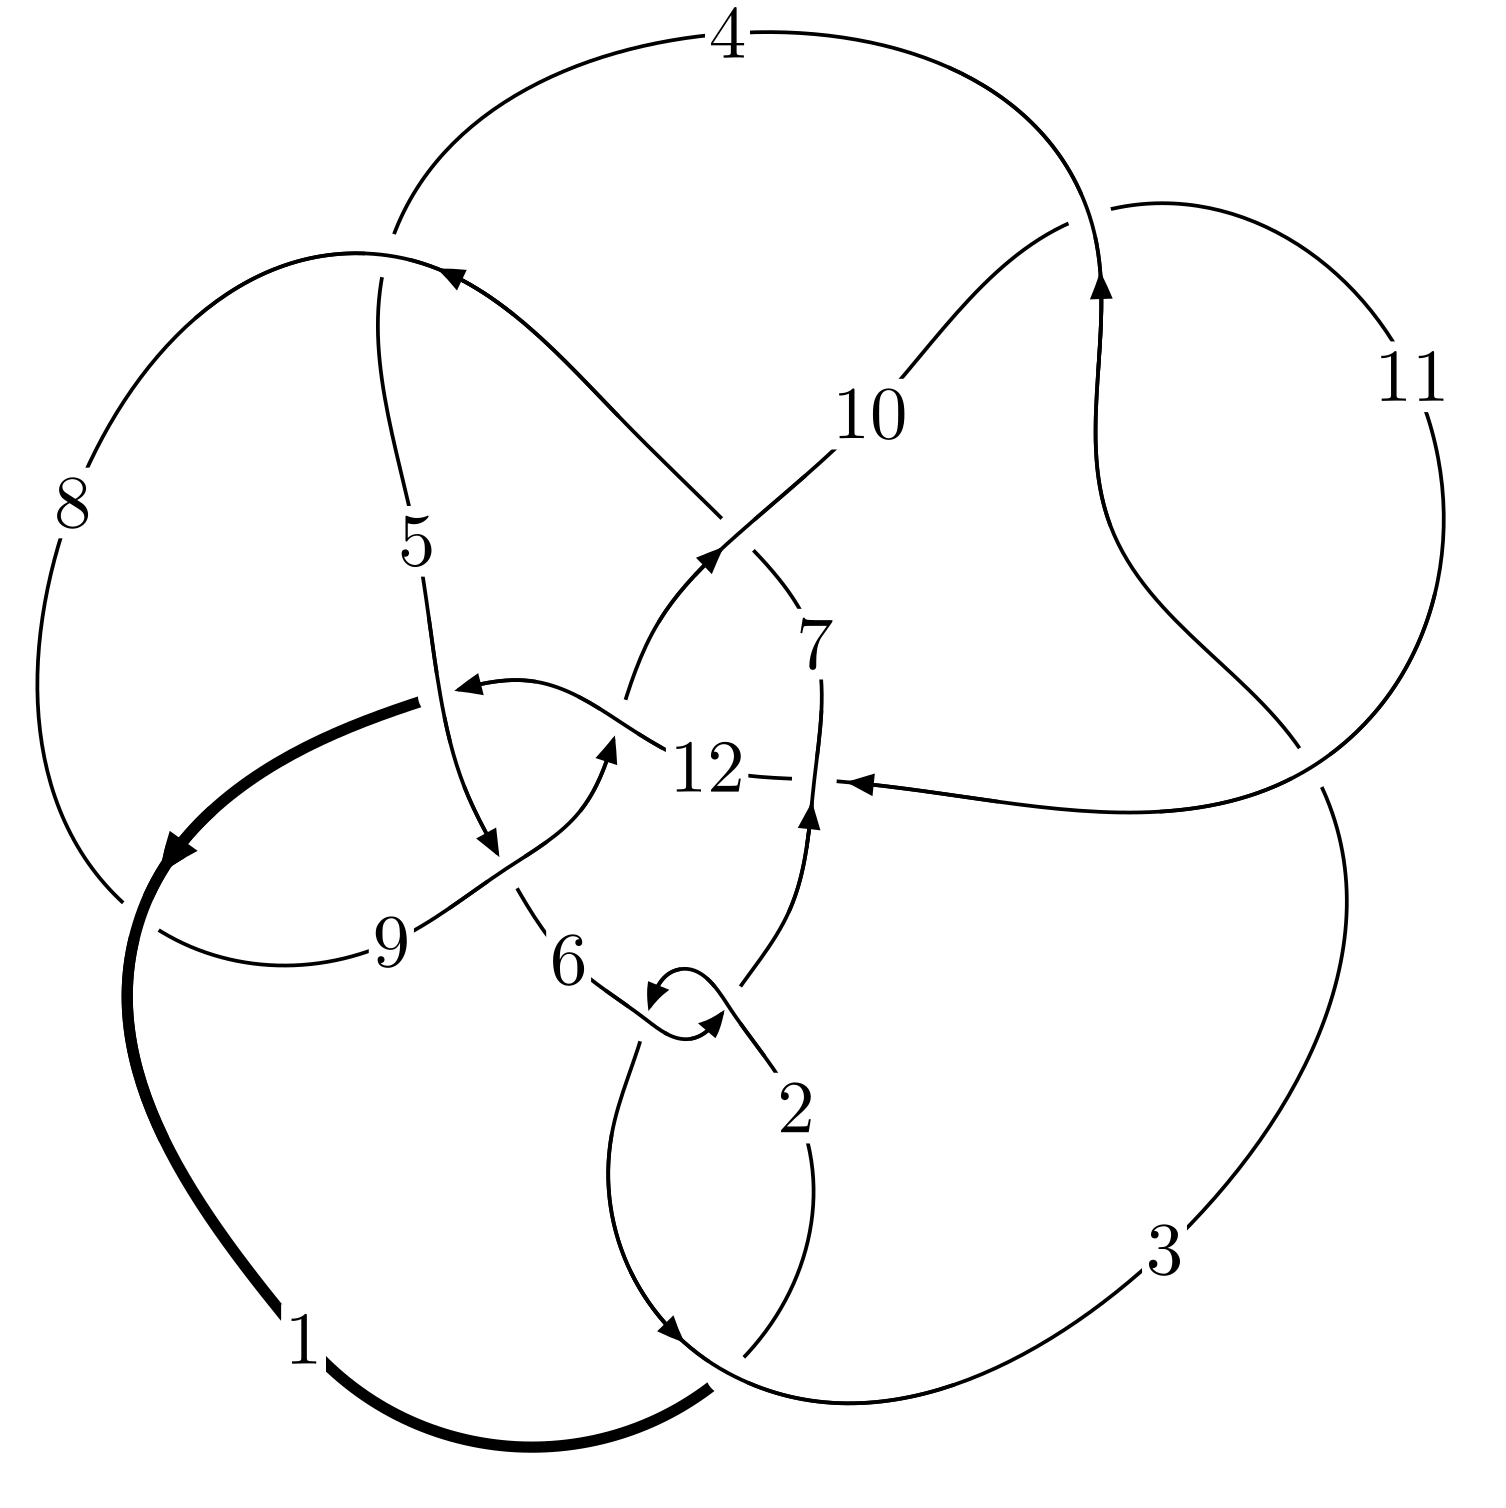
\includegraphics[width=112pt]{../../../GIT/diagram.site/Diagrams/png/1274_12a_0473.png}\\
\ \ \ A knot diagram\footnotemark}&
\allowdisplaybreaks
\textbf{Linearized knot diagam} \\
\cline{2-2}
 &
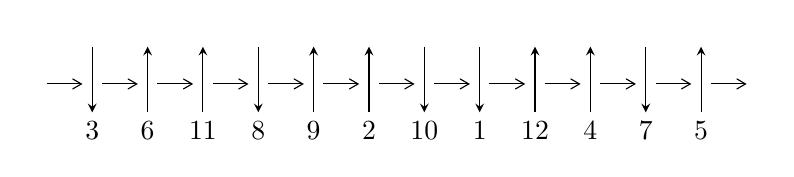
\begin{tikzpicture}[x=20pt, y=17pt]
	% nodes
	\node (C0) at (0, 0) {};
	\node (C1) at (1, 0) {};
	\node (C1U) at (1, +1) {};
	\node (C1D) at (1, -1) {3};

	\node (C2) at (2, 0) {};
	\node (C2U) at (2, +1) {};
	\node (C2D) at (2, -1) {6};

	\node (C3) at (3, 0) {};
	\node (C3U) at (3, +1) {};
	\node (C3D) at (3, -1) {11};

	\node (C4) at (4, 0) {};
	\node (C4U) at (4, +1) {};
	\node (C4D) at (4, -1) {8};

	\node (C5) at (5, 0) {};
	\node (C5U) at (5, +1) {};
	\node (C5D) at (5, -1) {9};

	\node (C6) at (6, 0) {};
	\node (C6U) at (6, +1) {};
	\node (C6D) at (6, -1) {2};

	\node (C7) at (7, 0) {};
	\node (C7U) at (7, +1) {};
	\node (C7D) at (7, -1) {10};

	\node (C8) at (8, 0) {};
	\node (C8U) at (8, +1) {};
	\node (C8D) at (8, -1) {1};

	\node (C9) at (9, 0) {};
	\node (C9U) at (9, +1) {};
	\node (C9D) at (9, -1) {12};

	\node (C10) at (10, 0) {};
	\node (C10U) at (10, +1) {};
	\node (C10D) at (10, -1) {4};

	\node (C11) at (11, 0) {};
	\node (C11U) at (11, +1) {};
	\node (C11D) at (11, -1) {7};

	\node (C12) at (12, 0) {};
	\node (C12U) at (12, +1) {};
	\node (C12D) at (12, -1) {5};
	\node (C13) at (13, 0) {};

	% arrows
	\draw[->,>={angle 60}]
	(C0) edge (C1) (C1) edge (C2) (C2) edge (C3) (C3) edge (C4) (C4) edge (C5) (C5) edge (C6) (C6) edge (C7) (C7) edge (C8) (C8) edge (C9) (C9) edge (C10) (C10) edge (C11) (C11) edge (C12) (C12) edge (C13) ;	\draw[->,>=stealth]
	(C1U) edge (C1D) (C2D) edge (C2U) (C3D) edge (C3U) (C4U) edge (C4D) (C5D) edge (C5U) (C6D) edge (C6U) (C7U) edge (C7D) (C8U) edge (C8D) (C9D) edge (C9U) (C10D) edge (C10U) (C11U) edge (C11D) (C12D) edge (C12U) ;
	\end{tikzpicture} \\
\hhline{~~} \\& 
\textbf{Solving Sequence} \\ \cline{2-2} 
 &
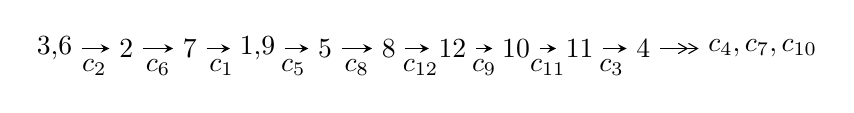
\begin{tikzpicture}[x=23pt, y=7pt]
	% node
	\node (A0) at (-1/8, 0) {3,6};
	\node (A1) at (1, 0) {2};
	\node (A2) at (2, 0) {7};
	\node (A3) at (49/16, 0) {1,9};
	\node (A4) at (33/8, 0) {5};
	\node (A5) at (41/8, 0) {8};
	\node (A6) at (49/8, 0) {12};
	\node (A7) at (57/8, 0) {10};
	\node (A8) at (65/8, 0) {11};
	\node (A9) at (73/8, 0) {4};
	\node (C1) at (1/2, -1) {$c_{2}$};
	\node (C2) at (3/2, -1) {$c_{6}$};
	\node (C3) at (5/2, -1) {$c_{1}$};
	\node (C4) at (29/8, -1) {$c_{5}$};
	\node (C5) at (37/8, -1) {$c_{8}$};
	\node (C6) at (45/8, -1) {$c_{12}$};
	\node (C7) at (53/8, -1) {$c_{9}$};
	\node (C8) at (61/8, -1) {$c_{11}$};
	\node (C9) at (69/8, -1) {$c_{3}$};
	\node (A10) at (11, 0) {$c_{4},c_{7},c_{10}$};

	% edge
	\draw[->,>=stealth]	
	(A0) edge (A1) (A1) edge (A2) (A2) edge (A3) (A3) edge (A4) (A4) edge (A5) (A5) edge (A6) (A6) edge (A7) (A7) edge (A8) (A8) edge (A9) ;
	\draw[->>,>={angle 60}]	
	(A9) edge (A10);
\end{tikzpicture} \\ 

\end{tabular} \\

\footnotetext{
The image of knot diagram is generated by the software ``\textbf{Draw programme}" developed by Andrew Bartholomew(\url{http://www.layer8.co.uk/maths/draw/index.htm\#Running-draw}), where we modified some parts for our purpose(\url{https://github.com/CATsTAILs/LinksPainter}).
}\phantom \\ \newline 
\centering \textbf{Ideals for irreducible components\footnotemark of $X_{\text{par}}$} 
 
\begin{align*}
I^u_{1}&=\langle 
-1.86496\times10^{672} u^{197}-1.78840\times10^{672} u^{196}+\cdots+1.18466\times10^{674} b+1.78262\times10^{673},\\
\phantom{I^u_{1}}&\phantom{= \langle  }2.32687\times10^{674} u^{197}+1.32190\times10^{674} u^{196}+\cdots+3.67245\times10^{675} a-1.48014\times10^{676},\\
\phantom{I^u_{1}}&\phantom{= \langle  }u^{198}+u^{197}+\cdots-192 u+31\rangle \\
I^u_{2}&=\langle 
2.58290\times10^{19} u^{53}-4.28590\times10^{19} u^{52}+\cdots+4.31513\times10^{17} b-5.83347\times10^{19},\\
\phantom{I^u_{2}}&\phantom{= \langle  }8.59240\times10^{18} u^{53}-1.13894\times10^{19} u^{52}+\cdots+4.31513\times10^{17} a-1.46351\times10^{19},\;u^{54}+17 u^{52}+\cdots+4 u+1\rangle \\
\\
\end{align*}
\raggedright * 2 irreducible components of $\dim_{\mathbb{C}}=0$, with total 252 representations.\\
\footnotetext{All coefficients of polynomials are rational numbers. But the coefficients are sometimes approximated in decimal forms when there is not enough margin.}
\newpage
\renewcommand{\arraystretch}{1}
\centering \section*{I. $I^u_{1}= \langle -1.86\times10^{672} u^{197}-1.79\times10^{672} u^{196}+\cdots+1.18\times10^{674} b+1.78\times10^{673},\;2.33\times10^{674} u^{197}+1.32\times10^{674} u^{196}+\cdots+3.67\times10^{675} a-1.48\times10^{676},\;u^{198}+u^{197}+\cdots-192 u+31 \rangle$}
\flushleft \textbf{(i) Arc colorings}\\
\begin{tabular}{m{7pt} m{180pt} m{7pt} m{180pt} }
\flushright $a_{3}=$&$\begin{pmatrix}1\\0\end{pmatrix}$ \\
\flushright $a_{6}=$&$\begin{pmatrix}0\\u\end{pmatrix}$ \\
\flushright $a_{2}=$&$\begin{pmatrix}1\\u^2\end{pmatrix}$ \\
\flushright $a_{7}=$&$\begin{pmatrix}u\\u^3+u\end{pmatrix}$ \\
\flushright $a_{1}=$&$\begin{pmatrix}u^2+1\\u^2\end{pmatrix}$ \\
\flushright $a_{9}=$&$\begin{pmatrix}-0.0633602 u^{197}-0.0359951 u^{196}+\cdots-20.8596 u+4.03040\\0.0157425 u^{197}+0.0150963 u^{196}+\cdots+1.94045 u-0.150475\end{pmatrix}$ \\
\flushright $a_{5}=$&$\begin{pmatrix}0.0677733 u^{197}+0.0199501 u^{196}+\cdots+12.6545 u+2.68158\\0.0290733 u^{197}-0.0351380 u^{196}+\cdots+4.67340 u-0.710225\end{pmatrix}$ \\
\flushright $a_{8}=$&$\begin{pmatrix}-0.0890583 u^{197}-0.0497108 u^{196}+\cdots-22.5654 u+4.17656\\0.0107942 u^{197}+0.00368821 u^{196}+\cdots+6.12461 u-0.722185\end{pmatrix}$ \\
\flushright $a_{12}=$&$\begin{pmatrix}0.0763840 u^{197}+0.0798270 u^{196}+\cdots-12.0972 u+3.22365\\-0.00122873 u^{197}+0.0100622 u^{196}+\cdots-1.09451 u-0.103854\end{pmatrix}$ \\
\flushright $a_{10}=$&$\begin{pmatrix}-0.00431990 u^{197}-0.0332907 u^{196}+\cdots+25.9650 u-4.73282\\0.0100152 u^{197}+0.0171788 u^{196}+\cdots+3.05089 u-0.0709769\end{pmatrix}$ \\
\flushright $a_{11}=$&$\begin{pmatrix}0.0633867 u^{197}+0.0532537 u^{196}+\cdots-10.4494 u+3.07203\\0.0124830 u^{197}+0.00627313 u^{196}+\cdots-1.65043 u+0.165386\end{pmatrix}$ \\
\flushright $a_{4}=$&$\begin{pmatrix}-0.0282330 u^{197}-0.0610010 u^{196}+\cdots+12.1616 u-1.21640\\0.0156224 u^{197}+0.0148252 u^{196}+\cdots+4.23594 u-0.550404\end{pmatrix}$\\&\end{tabular}
\flushleft \textbf{(ii) Obstruction class $= -1$}\\~\\
\flushleft \textbf{(iii) Cusp Shapes $= 0.0894793 u^{197}+0.286939 u^{196}+\cdots+37.0328 u-5.55261$}\\~\\
\newpage\renewcommand{\arraystretch}{1}
\flushleft \textbf{(iv) u-Polynomials at the component}\newline \\
\begin{tabular}{m{50pt}|m{274pt}}
Crossings & \hspace{64pt}u-Polynomials at each crossing \\
\hline $$\begin{aligned}c_{1}\end{aligned}$$&$\begin{aligned}
&u^{198}+103 u^{197}+\cdots+17448 u+961
\end{aligned}$\\
\hline $$\begin{aligned}c_{2},c_{6}\end{aligned}$$&$\begin{aligned}
&u^{198}- u^{197}+\cdots+192 u+31
\end{aligned}$\\
\hline $$\begin{aligned}c_{3},c_{10}\end{aligned}$$&$\begin{aligned}
&u^{198}+67 u^{196}+\cdots+33900 u+11483
\end{aligned}$\\
\hline $$\begin{aligned}c_{4}\end{aligned}$$&$\begin{aligned}
&u^{198}-50 u^{196}+\cdots-3343620599276 u+329813696659
\end{aligned}$\\
\hline $$\begin{aligned}c_{5}\end{aligned}$$&$\begin{aligned}
&u^{198}+u^{197}+\cdots-152 u+137
\end{aligned}$\\
\hline $$\begin{aligned}c_{7}\end{aligned}$$&$\begin{aligned}
&u^{198}+14 u^{197}+\cdots-3767846 u+4507105
\end{aligned}$\\
\hline $$\begin{aligned}c_{8}\end{aligned}$$&$\begin{aligned}
&u^{198}+5 u^{197}+\cdots-13533 u+913
\end{aligned}$\\
\hline $$\begin{aligned}c_{9}\end{aligned}$$&$\begin{aligned}
&u^{198}+14 u^{197}+\cdots+1162822100 u+97402681
\end{aligned}$\\
\hline $$\begin{aligned}c_{11}\end{aligned}$$&$\begin{aligned}
&u^{198}-2 u^{197}+\cdots+37555120 u+6187153
\end{aligned}$\\
\hline $$\begin{aligned}c_{12}\end{aligned}$$&$\begin{aligned}
&u^{198}-6 u^{197}+\cdots+13 u+1
\end{aligned}$\\
\hline
\end{tabular}\\~\\
\newpage\renewcommand{\arraystretch}{1}
\flushleft \textbf{(v) Riley Polynomials at the component}\newline \\
\begin{tabular}{m{50pt}|m{274pt}}
Crossings & \hspace{64pt}Riley Polynomials at each crossing \\
\hline $$\begin{aligned}c_{1}\end{aligned}$$&$\begin{aligned}
&y^{198}-5 y^{197}+\cdots+265997676 y+923521
\end{aligned}$\\
\hline $$\begin{aligned}c_{2},c_{6}\end{aligned}$$&$\begin{aligned}
&y^{198}+103 y^{197}+\cdots+17448 y+961
\end{aligned}$\\
\hline $$\begin{aligned}c_{3},c_{10}\end{aligned}$$&$\begin{aligned}
&y^{198}+134 y^{197}+\cdots+12295844278 y+131859289
\end{aligned}$\\
\hline $$\begin{aligned}c_{4}\end{aligned}$$&$\begin{aligned}
&y^{198}-100 y^{197}+\cdots-9.00\times10^{24} y+1.09\times10^{23}
\end{aligned}$\\
\hline $$\begin{aligned}c_{5}\end{aligned}$$&$\begin{aligned}
&y^{198}+25 y^{197}+\cdots+1495404 y+18769
\end{aligned}$\\
\hline $$\begin{aligned}c_{7}\end{aligned}$$&$\begin{aligned}
&y^{198}-80 y^{197}+\cdots-1202038047552706 y+20313995481025
\end{aligned}$\\
\hline $$\begin{aligned}c_{8}\end{aligned}$$&$\begin{aligned}
&y^{198}-45 y^{197}+\cdots+443152173 y+833569
\end{aligned}$\\
\hline $$\begin{aligned}c_{9}\end{aligned}$$&$\begin{aligned}
&y^{198}+44 y^{197}+\cdots+370665595377026344 y+9487282265987761
\end{aligned}$\\
\hline $$\begin{aligned}c_{11}\end{aligned}$$&$\begin{aligned}
&y^{198}-56 y^{197}+\cdots+6038753260673846 y+38280862245409
\end{aligned}$\\
\hline $$\begin{aligned}c_{12}\end{aligned}$$&$\begin{aligned}
&y^{198}+32 y^{197}+\cdots+265 y+1
\end{aligned}$\\
\hline
\end{tabular}\\~\\
\newpage\flushleft \textbf{(vi) Complex Volumes and Cusp Shapes}
$$\begin{array}{c|c|c}  
\text{Solutions to }I^u_{1}& \I (\text{vol} + \sqrt{-1}CS) & \text{Cusp shape}\\
 \hline 
\begin{aligned}
u &= -0.824810 + 0.553156 I \\
a &= -0.69533 + 1.41516 I \\
b &= -0.284646 + 0.141860 I\end{aligned}
 & -3.58312 - 3.95709 I & \phantom{-0.000000 } 0 \\ \hline\begin{aligned}
u &= -0.824810 - 0.553156 I \\
a &= -0.69533 - 1.41516 I \\
b &= -0.284646 - 0.141860 I\end{aligned}
 & -3.58312 + 3.95709 I & \phantom{-0.000000 } 0 \\ \hline\begin{aligned}
u &= -0.963257 + 0.293593 I \\
a &= \phantom{-}0.70929 + 1.40633 I \\
b &= \phantom{-}1.339760 + 0.216023 I\end{aligned}
 & -4.5956 + 15.6769 I & \phantom{-0.000000 } 0 \\ \hline\begin{aligned}
u &= -0.963257 - 0.293593 I \\
a &= \phantom{-}0.70929 - 1.40633 I \\
b &= \phantom{-}1.339760 - 0.216023 I\end{aligned}
 & -4.5956 - 15.6769 I & \phantom{-0.000000 } 0 \\ \hline\begin{aligned}
u &= -0.729511 + 0.724454 I \\
a &= -1.066650 - 0.355340 I \\
b &= -1.09557 + 0.99016 I\end{aligned}
 & \phantom{-}2.59433 - 0.83840 I & \phantom{-0.000000 } 0 \\ \hline\begin{aligned}
u &= -0.729511 - 0.724454 I \\
a &= -1.066650 + 0.355340 I \\
b &= -1.09557 - 0.99016 I\end{aligned}
 & \phantom{-}2.59433 + 0.83840 I & \phantom{-0.000000 } 0 \\ \hline\begin{aligned}
u &= -0.381241 + 0.956773 I \\
a &= -0.555354 + 0.662424 I \\
b &= \phantom{-}0.563657 + 0.070525 I\end{aligned}
 & -0.93368 - 2.82399 I & \phantom{-0.000000 } 0 \\ \hline\begin{aligned}
u &= -0.381241 - 0.956773 I \\
a &= -0.555354 - 0.662424 I \\
b &= \phantom{-}0.563657 - 0.070525 I\end{aligned}
 & -0.93368 + 2.82399 I & \phantom{-0.000000 } 0 \\ \hline\begin{aligned}
u &= \phantom{-}0.877338 + 0.412580 I \\
a &= \phantom{-}0.47161 - 1.33895 I \\
b &= \phantom{-}1.232260 - 0.166680 I\end{aligned}
 & \phantom{-}0.06938 - 4.33235 I & \phantom{-0.000000 } 0 \\ \hline\begin{aligned}
u &= \phantom{-}0.877338 - 0.412580 I \\
a &= \phantom{-}0.47161 + 1.33895 I \\
b &= \phantom{-}1.232260 + 0.166680 I\end{aligned}
 & \phantom{-}0.06938 + 4.33235 I & \phantom{-0.000000 } 0\\
 \hline 
 \end{array}$$\newpage$$\begin{array}{c|c|c}  
\text{Solutions to }I^u_{1}& \I (\text{vol} + \sqrt{-1}CS) & \text{Cusp shape}\\
 \hline 
\begin{aligned}
u &= -0.222610 + 1.006240 I \\
a &= \phantom{-}0.406687 - 0.257500 I \\
b &= \phantom{-}3.08749 - 2.46706 I\end{aligned}
 & -8.49476 - 5.37600 I & \phantom{-0.000000 } 0 \\ \hline\begin{aligned}
u &= -0.222610 - 1.006240 I \\
a &= \phantom{-}0.406687 + 0.257500 I \\
b &= \phantom{-}3.08749 + 2.46706 I\end{aligned}
 & -8.49476 + 5.37600 I & \phantom{-0.000000 } 0 \\ \hline\begin{aligned}
u &= \phantom{-}0.802811 + 0.538722 I \\
a &= \phantom{-}1.188090 + 0.731574 I \\
b &= \phantom{-}1.260460 + 0.278506 I\end{aligned}
 & -4.06775 + 3.53850 I & \phantom{-0.000000 } 0 \\ \hline\begin{aligned}
u &= \phantom{-}0.802811 - 0.538722 I \\
a &= \phantom{-}1.188090 - 0.731574 I \\
b &= \phantom{-}1.260460 - 0.278506 I\end{aligned}
 & -4.06775 - 3.53850 I & \phantom{-0.000000 } 0 \\ \hline\begin{aligned}
u &= \phantom{-}0.255685 + 1.005100 I \\
a &= \phantom{-}0.738611 + 0.326309 I \\
b &= -1.114180 - 0.226089 I\end{aligned}
 & -4.83208 + 5.96241 I & \phantom{-0.000000 } 0 \\ \hline\begin{aligned}
u &= \phantom{-}0.255685 - 1.005100 I \\
a &= \phantom{-}0.738611 - 0.326309 I \\
b &= -1.114180 + 0.226089 I\end{aligned}
 & -4.83208 - 5.96241 I & \phantom{-0.000000 } 0 \\ \hline\begin{aligned}
u &= -0.254005 + 1.014770 I \\
a &= -0.786575 + 0.268218 I \\
b &= -1.25127 - 1.19822 I\end{aligned}
 & -8.14733 - 0.80174 I & \phantom{-0.000000 } 0 \\ \hline\begin{aligned}
u &= -0.254005 - 1.014770 I \\
a &= -0.786575 - 0.268218 I \\
b &= -1.25127 + 1.19822 I\end{aligned}
 & -8.14733 + 0.80174 I & \phantom{-0.000000 } 0 \\ \hline\begin{aligned}
u &= \phantom{-}0.236003 + 1.019580 I \\
a &= \phantom{-}1.123630 + 0.673011 I \\
b &= \phantom{-}1.44734 + 1.25988 I\end{aligned}
 & -4.68178 - 4.39747 I & \phantom{-0.000000 } 0 \\ \hline\begin{aligned}
u &= \phantom{-}0.236003 - 1.019580 I \\
a &= \phantom{-}1.123630 - 0.673011 I \\
b &= \phantom{-}1.44734 - 1.25988 I\end{aligned}
 & -4.68178 + 4.39747 I & \phantom{-0.000000 } 0\\
 \hline 
 \end{array}$$\newpage$$\begin{array}{c|c|c}  
\text{Solutions to }I^u_{1}& \I (\text{vol} + \sqrt{-1}CS) & \text{Cusp shape}\\
 \hline 
\begin{aligned}
u &= -0.132449 + 1.039490 I \\
a &= \phantom{-}0.915902 + 0.468946 I \\
b &= \phantom{-}1.76687 + 0.09225 I\end{aligned}
 & -4.76977 - 4.96050 I & \phantom{-0.000000 } 0 \\ \hline\begin{aligned}
u &= -0.132449 - 1.039490 I \\
a &= \phantom{-}0.915902 - 0.468946 I \\
b &= \phantom{-}1.76687 - 0.09225 I\end{aligned}
 & -4.76977 + 4.96050 I & \phantom{-0.000000 } 0 \\ \hline\begin{aligned}
u &= \phantom{-}0.614386 + 0.715810 I \\
a &= -0.378979 + 1.009620 I \\
b &= -1.56433 + 0.11301 I\end{aligned}
 & \phantom{-}4.21166 - 0.54080 I & \phantom{-0.000000 } 0 \\ \hline\begin{aligned}
u &= \phantom{-}0.614386 - 0.715810 I \\
a &= -0.378979 - 1.009620 I \\
b &= -1.56433 - 0.11301 I\end{aligned}
 & \phantom{-}4.21166 + 0.54080 I & \phantom{-0.000000 } 0 \\ \hline\begin{aligned}
u &= \phantom{-}0.594908 + 0.878745 I \\
a &= \phantom{-}1.032970 - 0.515434 I \\
b &= \phantom{-}1.30871 + 1.42246 I\end{aligned}
 & \phantom{-}3.73146 + 5.29164 I & \phantom{-0.000000 } 0 \\ \hline\begin{aligned}
u &= \phantom{-}0.594908 - 0.878745 I \\
a &= \phantom{-}1.032970 + 0.515434 I \\
b &= \phantom{-}1.30871 - 1.42246 I\end{aligned}
 & \phantom{-}3.73146 - 5.29164 I & \phantom{-0.000000 } 0 \\ \hline\begin{aligned}
u &= \phantom{-}1.039900 + 0.228021 I \\
a &= -0.226420 + 0.522952 I \\
b &= -0.478681 + 0.172308 I\end{aligned}
 & -3.45727 - 6.87757 I & \phantom{-0.000000 } 0 \\ \hline\begin{aligned}
u &= \phantom{-}1.039900 - 0.228021 I \\
a &= -0.226420 - 0.522952 I \\
b &= -0.478681 - 0.172308 I\end{aligned}
 & -3.45727 + 6.87757 I & \phantom{-0.000000 } 0 \\ \hline\begin{aligned}
u &= -0.737283 + 0.564655 I \\
a &= -1.52356 - 0.00658 I \\
b &= -0.924037 + 0.911189 I\end{aligned}
 & \phantom{-}0.51049 - 3.80248 I & \phantom{-0.000000 } 0 \\ \hline\begin{aligned}
u &= -0.737283 - 0.564655 I \\
a &= -1.52356 + 0.00658 I \\
b &= -0.924037 - 0.911189 I\end{aligned}
 & \phantom{-}0.51049 + 3.80248 I & \phantom{-0.000000 } 0\\
 \hline 
 \end{array}$$\newpage$$\begin{array}{c|c|c}  
\text{Solutions to }I^u_{1}& \I (\text{vol} + \sqrt{-1}CS) & \text{Cusp shape}\\
 \hline 
\begin{aligned}
u &= \phantom{-}0.416017 + 0.993053 I \\
a &= \phantom{-}0.720929 + 0.437955 I \\
b &= \phantom{-}1.166810 - 0.354621 I\end{aligned}
 & -3.38687 + 1.35108 I & \phantom{-0.000000 } 0 \\ \hline\begin{aligned}
u &= \phantom{-}0.416017 - 0.993053 I \\
a &= \phantom{-}0.720929 - 0.437955 I \\
b &= \phantom{-}1.166810 + 0.354621 I\end{aligned}
 & -3.38687 - 1.35108 I & \phantom{-0.000000 } 0 \\ \hline\begin{aligned}
u &= \phantom{-}0.232488 + 1.052280 I \\
a &= -0.799893 + 1.019930 I \\
b &= -2.76987 - 1.73929 I\end{aligned}
 & -8.89238 + 5.32591 I & \phantom{-0.000000 } 0 \\ \hline\begin{aligned}
u &= \phantom{-}0.232488 - 1.052280 I \\
a &= -0.799893 - 1.019930 I \\
b &= -2.76987 + 1.73929 I\end{aligned}
 & -8.89238 - 5.32591 I & \phantom{-0.000000 } 0 \\ \hline\begin{aligned}
u &= -0.279734 + 1.040910 I \\
a &= -0.253261 + 0.176642 I \\
b &= -3.07992 + 2.05683 I\end{aligned}
 & -8.82880 + 3.92495 I & \phantom{-0.000000 } 0 \\ \hline\begin{aligned}
u &= -0.279734 - 1.040910 I \\
a &= -0.253261 - 0.176642 I \\
b &= -3.07992 - 2.05683 I\end{aligned}
 & -8.82880 - 3.92495 I & \phantom{-0.000000 } 0 \\ \hline\begin{aligned}
u &= \phantom{-}0.486449 + 0.961931 I \\
a &= \phantom{-}0.185939 + 0.008126 I \\
b &= \phantom{-}1.70735 + 0.50992 I\end{aligned}
 & -1.97977 - 0.72064 I & \phantom{-0.000000 } 0 \\ \hline\begin{aligned}
u &= \phantom{-}0.486449 - 0.961931 I \\
a &= \phantom{-}0.185939 - 0.008126 I \\
b &= \phantom{-}1.70735 - 0.50992 I\end{aligned}
 & -1.97977 + 0.72064 I & \phantom{-0.000000 } 0 \\ \hline\begin{aligned}
u &= \phantom{-}0.847298 + 0.351445 I \\
a &= -0.65649 + 1.50631 I \\
b &= -1.39353 + 0.24812 I\end{aligned}
 & -0.33300 - 9.63949 I & \phantom{-0.000000 } 0 \\ \hline\begin{aligned}
u &= \phantom{-}0.847298 - 0.351445 I \\
a &= -0.65649 - 1.50631 I \\
b &= -1.39353 - 0.24812 I\end{aligned}
 & -0.33300 + 9.63949 I & \phantom{-0.000000 } 0\\
 \hline 
 \end{array}$$\newpage$$\begin{array}{c|c|c}  
\text{Solutions to }I^u_{1}& \I (\text{vol} + \sqrt{-1}CS) & \text{Cusp shape}\\
 \hline 
\begin{aligned}
u &= \phantom{-}0.384297 + 1.022610 I \\
a &= \phantom{-}0.915893 + 0.258477 I \\
b &= \phantom{-}0.591419 - 0.583888 I\end{aligned}
 & -7.60838 + 5.05242 I & \phantom{-0.000000 } 0 \\ \hline\begin{aligned}
u &= \phantom{-}0.384297 - 1.022610 I \\
a &= \phantom{-}0.915893 - 0.258477 I \\
b &= \phantom{-}0.591419 + 0.583888 I\end{aligned}
 & -7.60838 - 5.05242 I & \phantom{-0.000000 } 0 \\ \hline\begin{aligned}
u &= -0.394959 + 1.023850 I \\
a &= -1.19575 + 1.09283 I \\
b &= -0.44012 + 1.55630 I\end{aligned}
 & -1.48905 + 0.43411 I & \phantom{-0.000000 } 0 \\ \hline\begin{aligned}
u &= -0.394959 - 1.023850 I \\
a &= -1.19575 - 1.09283 I \\
b &= -0.44012 - 1.55630 I\end{aligned}
 & -1.48905 - 0.43411 I & \phantom{-0.000000 } 0 \\ \hline\begin{aligned}
u &= \phantom{-}0.251533 + 1.071030 I \\
a &= \phantom{-}0.92596 - 1.18051 I \\
b &= \phantom{-}2.97705 + 0.89424 I\end{aligned}
 & -8.96847 - 4.35509 I & \phantom{-0.000000 } 0 \\ \hline\begin{aligned}
u &= \phantom{-}0.251533 - 1.071030 I \\
a &= \phantom{-}0.92596 + 1.18051 I \\
b &= \phantom{-}2.97705 - 0.89424 I\end{aligned}
 & -8.96847 + 4.35509 I & \phantom{-0.000000 } 0 \\ \hline\begin{aligned}
u &= -0.812119 + 0.745419 I \\
a &= \phantom{-}0.895161 + 0.236677 I \\
b &= \phantom{-}0.762848 - 0.865532 I\end{aligned}
 & \phantom{-}1.80790 - 6.18377 I & \phantom{-0.000000 } 0 \\ \hline\begin{aligned}
u &= -0.812119 - 0.745419 I \\
a &= \phantom{-}0.895161 - 0.236677 I \\
b &= \phantom{-}0.762848 + 0.865532 I\end{aligned}
 & \phantom{-}1.80790 + 6.18377 I & \phantom{-0.000000 } 0 \\ \hline\begin{aligned}
u &= -0.372855 + 1.039690 I \\
a &= -0.968646 + 0.800400 I \\
b &= -1.172610 + 0.172507 I\end{aligned}
 & -7.23762 + 3.27750 I & \phantom{-0.000000 } 0 \\ \hline\begin{aligned}
u &= -0.372855 - 1.039690 I \\
a &= -0.968646 - 0.800400 I \\
b &= -1.172610 - 0.172507 I\end{aligned}
 & -7.23762 - 3.27750 I & \phantom{-0.000000 } 0\\
 \hline 
 \end{array}$$\newpage$$\begin{array}{c|c|c}  
\text{Solutions to }I^u_{1}& \I (\text{vol} + \sqrt{-1}CS) & \text{Cusp shape}\\
 \hline 
\begin{aligned}
u &= \phantom{-}0.519911 + 0.722424 I \\
a &= -0.026612 - 0.141068 I \\
b &= \phantom{-}1.108450 + 0.675080 I\end{aligned}
 & -1.83814 - 0.88802 I & \phantom{-0.000000 } 0 \\ \hline\begin{aligned}
u &= \phantom{-}0.519911 - 0.722424 I \\
a &= -0.026612 + 0.141068 I \\
b &= \phantom{-}1.108450 - 0.675080 I\end{aligned}
 & -1.83814 + 0.88802 I & \phantom{-0.000000 } 0 \\ \hline\begin{aligned}
u &= -1.046270 + 0.379600 I \\
a &= -0.053059 + 0.358438 I \\
b &= \phantom{-}0.155168 + 0.269625 I\end{aligned}
 & \phantom{-}0.565986 + 0.651189 I & \phantom{-0.000000 } 0 \\ \hline\begin{aligned}
u &= -1.046270 - 0.379600 I \\
a &= -0.053059 - 0.358438 I \\
b &= \phantom{-}0.155168 - 0.269625 I\end{aligned}
 & \phantom{-}0.565986 - 0.651189 I & \phantom{-0.000000 } 0 \\ \hline\begin{aligned}
u &= -0.683256 + 0.893934 I \\
a &= \phantom{-}0.332044 + 0.846280 I \\
b &= \phantom{-}1.381190 + 0.089150 I\end{aligned}
 & \phantom{-}2.08908 - 4.49974 I & \phantom{-0.000000 } 0 \\ \hline\begin{aligned}
u &= -0.683256 - 0.893934 I \\
a &= \phantom{-}0.332044 - 0.846280 I \\
b &= \phantom{-}1.381190 - 0.089150 I\end{aligned}
 & \phantom{-}2.08908 + 4.49974 I & \phantom{-0.000000 } 0 \\ \hline\begin{aligned}
u &= \phantom{-}0.485445 + 1.016770 I \\
a &= -0.524205 + 0.003433 I \\
b &= -1.67733 - 1.65044 I\end{aligned}
 & -2.96479 + 4.78008 I & \phantom{-0.000000 } 0 \\ \hline\begin{aligned}
u &= \phantom{-}0.485445 - 1.016770 I \\
a &= -0.524205 - 0.003433 I \\
b &= -1.67733 + 1.65044 I\end{aligned}
 & -2.96479 - 4.78008 I & \phantom{-0.000000 } 0 \\ \hline\begin{aligned}
u &= -0.444508 + 1.039410 I \\
a &= -1.50105 - 0.95204 I \\
b &= -2.42661 + 1.25090 I\end{aligned}
 & -3.24317 - 1.20456 I & \phantom{-0.000000 } 0 \\ \hline\begin{aligned}
u &= -0.444508 - 1.039410 I \\
a &= -1.50105 + 0.95204 I \\
b &= -2.42661 - 1.25090 I\end{aligned}
 & -3.24317 + 1.20456 I & \phantom{-0.000000 } 0\\
 \hline 
 \end{array}$$\newpage$$\begin{array}{c|c|c}  
\text{Solutions to }I^u_{1}& \I (\text{vol} + \sqrt{-1}CS) & \text{Cusp shape}\\
 \hline 
\begin{aligned}
u &= -0.308845 + 1.088940 I \\
a &= \phantom{-}0.370261 - 0.776912 I \\
b &= -0.084035 + 1.029990 I\end{aligned}
 & -5.84447 + 4.04897 I & \phantom{-0.000000 } 0 \\ \hline\begin{aligned}
u &= -0.308845 - 1.088940 I \\
a &= \phantom{-}0.370261 + 0.776912 I \\
b &= -0.084035 - 1.029990 I\end{aligned}
 & -5.84447 - 4.04897 I & \phantom{-0.000000 } 0 \\ \hline\begin{aligned}
u &= -0.518948 + 1.011330 I \\
a &= \phantom{-}0.310847 + 1.039890 I \\
b &= \phantom{-}1.56683 - 0.36672 I\end{aligned}
 & -0.39175 - 2.63542 I & \phantom{-0.000000 } 0 \\ \hline\begin{aligned}
u &= -0.518948 - 1.011330 I \\
a &= \phantom{-}0.310847 - 1.039890 I \\
b &= \phantom{-}1.56683 + 0.36672 I\end{aligned}
 & -0.39175 + 2.63542 I & \phantom{-0.000000 } 0 \\ \hline\begin{aligned}
u &= \phantom{-}0.462927 + 1.047690 I \\
a &= \phantom{-}0.288225 - 0.977650 I \\
b &= \phantom{-}1.27654 + 1.30182 I\end{aligned}
 & \phantom{-}1.25206 + 3.28632 I & \phantom{-0.000000 } 0 \\ \hline\begin{aligned}
u &= \phantom{-}0.462927 - 1.047690 I \\
a &= \phantom{-}0.288225 + 0.977650 I \\
b &= \phantom{-}1.27654 - 1.30182 I\end{aligned}
 & \phantom{-}1.25206 - 3.28632 I & \phantom{-0.000000 } 0 \\ \hline\begin{aligned}
u &= -1.141360 + 0.146277 I \\
a &= -0.87484 - 1.20045 I \\
b &= -1.232320 - 0.216989 I\end{aligned}
 & -2.16615 + 5.60711 I & \phantom{-0.000000 } 0 \\ \hline\begin{aligned}
u &= -1.141360 - 0.146277 I \\
a &= -0.87484 + 1.20045 I \\
b &= -1.232320 + 0.216989 I\end{aligned}
 & -2.16615 - 5.60711 I & \phantom{-0.000000 } 0 \\ \hline\begin{aligned}
u &= -0.762448 + 0.373427 I \\
a &= \phantom{-}0.001253 - 0.627888 I \\
b &= -0.994084 + 0.270184 I\end{aligned}
 & -3.64779 + 1.26818 I & \phantom{-0.000000 } 0 \\ \hline\begin{aligned}
u &= -0.762448 - 0.373427 I \\
a &= \phantom{-}0.001253 + 0.627888 I \\
b &= -0.994084 - 0.270184 I\end{aligned}
 & -3.64779 - 1.26818 I & \phantom{-0.000000 } 0\\
 \hline 
 \end{array}$$\newpage$$\begin{array}{c|c|c}  
\text{Solutions to }I^u_{1}& \I (\text{vol} + \sqrt{-1}CS) & \text{Cusp shape}\\
 \hline 
\begin{aligned}
u &= \phantom{-}0.747516 + 0.402468 I \\
a &= \phantom{-}0.21934 - 1.93663 I \\
b &= \phantom{-}1.108420 - 0.191050 I\end{aligned}
 & -0.20396 - 6.41614 I & \phantom{-0.000000 } 0 \\ \hline\begin{aligned}
u &= \phantom{-}0.747516 - 0.402468 I \\
a &= \phantom{-}0.21934 + 1.93663 I \\
b &= \phantom{-}1.108420 + 0.191050 I\end{aligned}
 & -0.20396 + 6.41614 I & \phantom{-0.000000 } 0 \\ \hline\begin{aligned}
u &= -0.377232 + 1.089410 I \\
a &= \phantom{-}0.797220 - 1.067190 I \\
b &= \phantom{-}0.104841 - 0.329076 I\end{aligned}
 & -8.66867 + 0.54381 I & \phantom{-0.000000 } 0 \\ \hline\begin{aligned}
u &= -0.377232 - 1.089410 I \\
a &= \phantom{-}0.797220 + 1.067190 I \\
b &= \phantom{-}0.104841 + 0.329076 I\end{aligned}
 & -8.66867 - 0.54381 I & \phantom{-0.000000 } 0 \\ \hline\begin{aligned}
u &= \phantom{-}0.489049 + 1.044700 I \\
a &= -0.664690 + 0.020529 I \\
b &= -1.97839 + 0.09531 I\end{aligned}
 & -1.45922 + 6.72358 I & \phantom{-0.000000 } 0 \\ \hline\begin{aligned}
u &= \phantom{-}0.489049 - 1.044700 I \\
a &= -0.664690 - 0.020529 I \\
b &= -1.97839 - 0.09531 I\end{aligned}
 & -1.45922 - 6.72358 I & \phantom{-0.000000 } 0 \\ \hline\begin{aligned}
u &= \phantom{-}0.245589 + 1.127890 I \\
a &= -0.870344 - 0.754624 I \\
b &= \phantom{-}0.251260 - 1.202110 I\end{aligned}
 & -8.93341 + 0.08390 I & \phantom{-0.000000 } 0 \\ \hline\begin{aligned}
u &= \phantom{-}0.245589 - 1.127890 I \\
a &= -0.870344 + 0.754624 I \\
b &= \phantom{-}0.251260 + 1.202110 I\end{aligned}
 & -8.93341 - 0.08390 I & \phantom{-0.000000 } 0 \\ \hline\begin{aligned}
u &= -0.472608 + 1.055410 I \\
a &= \phantom{-}0.97037 - 1.55840 I \\
b &= -0.58648 - 1.59176 I\end{aligned}
 & -3.01128 - 5.39837 I & \phantom{-0.000000 } 0 \\ \hline\begin{aligned}
u &= -0.472608 - 1.055410 I \\
a &= \phantom{-}0.97037 + 1.55840 I \\
b &= -0.58648 + 1.59176 I\end{aligned}
 & -3.01128 + 5.39837 I & \phantom{-0.000000 } 0\\
 \hline 
 \end{array}$$\newpage$$\begin{array}{c|c|c}  
\text{Solutions to }I^u_{1}& \I (\text{vol} + \sqrt{-1}CS) & \text{Cusp shape}\\
 \hline 
\begin{aligned}
u &= \phantom{-}0.757260 + 0.364751 I \\
a &= -2.12506 - 0.90755 I \\
b &= -1.19865 - 0.83244 I\end{aligned}
 & -4.53758 - 6.76051 I & \phantom{-0.000000 } 0 \\ \hline\begin{aligned}
u &= \phantom{-}0.757260 - 0.364751 I \\
a &= -2.12506 + 0.90755 I \\
b &= -1.19865 + 0.83244 I\end{aligned}
 & -4.53758 + 6.76051 I & \phantom{-0.000000 } 0 \\ \hline\begin{aligned}
u &= \phantom{-}0.364061 + 1.102010 I \\
a &= -1.026340 - 0.363460 I \\
b &= -0.328856 - 0.468998 I\end{aligned}
 & -8.23780 + 7.37982 I & \phantom{-0.000000 } 0 \\ \hline\begin{aligned}
u &= \phantom{-}0.364061 - 1.102010 I \\
a &= -1.026340 + 0.363460 I \\
b &= -0.328856 + 0.468998 I\end{aligned}
 & -8.23780 - 7.37982 I & \phantom{-0.000000 } 0 \\ \hline\begin{aligned}
u &= \phantom{-}0.522730 + 1.037170 I \\
a &= -0.378495 - 0.177136 I \\
b &= -0.18124 - 1.46254 I\end{aligned}
 & -6.63260 + 1.33254 I & \phantom{-0.000000 } 0 \\ \hline\begin{aligned}
u &= \phantom{-}0.522730 - 1.037170 I \\
a &= -0.378495 + 0.177136 I \\
b &= -0.18124 + 1.46254 I\end{aligned}
 & -6.63260 - 1.33254 I & \phantom{-0.000000 } 0 \\ \hline\begin{aligned}
u &= \phantom{-}0.265860 + 1.133190 I \\
a &= \phantom{-}0.495368 + 0.624719 I \\
b &= \phantom{-}0.637140 + 0.235968 I\end{aligned}
 & -4.39155 + 0.24998 I & \phantom{-0.000000 } 0 \\ \hline\begin{aligned}
u &= \phantom{-}0.265860 - 1.133190 I \\
a &= \phantom{-}0.495368 - 0.624719 I \\
b &= \phantom{-}0.637140 - 0.235968 I\end{aligned}
 & -4.39155 - 0.24998 I & \phantom{-0.000000 } 0 \\ \hline\begin{aligned}
u &= \phantom{-}0.599728 + 0.577169 I \\
a &= -0.388694 + 0.200588 I \\
b &= -0.28828 - 1.44371 I\end{aligned}
 & -0.91719 + 5.13630 I & \phantom{-0.000000 } 0 \\ \hline\begin{aligned}
u &= \phantom{-}0.599728 - 0.577169 I \\
a &= -0.388694 - 0.200588 I \\
b &= -0.28828 + 1.44371 I\end{aligned}
 & -0.91719 - 5.13630 I & \phantom{-0.000000 } 0\\
 \hline 
 \end{array}$$\newpage$$\begin{array}{c|c|c}  
\text{Solutions to }I^u_{1}& \I (\text{vol} + \sqrt{-1}CS) & \text{Cusp shape}\\
 \hline 
\begin{aligned}
u &= \phantom{-}0.782592 + 0.282194 I \\
a &= -1.11690 + 1.37447 I \\
b &= -1.075150 + 0.342609 I\end{aligned}
 & -4.38008 - 2.89098 I & \phantom{-0.000000 } 0 \\ \hline\begin{aligned}
u &= \phantom{-}0.782592 - 0.282194 I \\
a &= -1.11690 - 1.37447 I \\
b &= -1.075150 - 0.342609 I\end{aligned}
 & -4.38008 + 2.89098 I & \phantom{-0.000000 } 0 \\ \hline\begin{aligned}
u &= -0.500040 + 1.059690 I \\
a &= \phantom{-}1.70534 + 0.45569 I \\
b &= \phantom{-}2.51555 - 1.68935 I\end{aligned}
 & -0.73399 - 7.01501 I & \phantom{-0.000000 } 0 \\ \hline\begin{aligned}
u &= -0.500040 - 1.059690 I \\
a &= \phantom{-}1.70534 - 0.45569 I \\
b &= \phantom{-}2.51555 + 1.68935 I\end{aligned}
 & -0.73399 + 7.01501 I & \phantom{-0.000000 } 0 \\ \hline\begin{aligned}
u &= -0.639301 + 0.983530 I \\
a &= \phantom{-}0.197767 + 1.128470 I \\
b &= \phantom{-}1.156070 + 0.411848 I\end{aligned}
 & -0.72364 - 1.41803 I & \phantom{-0.000000 } 0 \\ \hline\begin{aligned}
u &= -0.639301 - 0.983530 I \\
a &= \phantom{-}0.197767 - 1.128470 I \\
b &= \phantom{-}1.156070 - 0.411848 I\end{aligned}
 & -0.72364 + 1.41803 I & \phantom{-0.000000 } 0 \\ \hline\begin{aligned}
u &= -0.723369 + 0.387062 I \\
a &= \phantom{-}0.242751 - 0.938498 I \\
b &= \phantom{-}0.610791 + 0.843374 I\end{aligned}
 & -4.67901 + 6.09919 I & \phantom{-0.000000 } 0 \\ \hline\begin{aligned}
u &= -0.723369 - 0.387062 I \\
a &= \phantom{-}0.242751 + 0.938498 I \\
b &= \phantom{-}0.610791 - 0.843374 I\end{aligned}
 & -4.67901 - 6.09919 I & \phantom{-0.000000 } 0 \\ \hline\begin{aligned}
u &= -0.020576 + 1.185450 I \\
a &= \phantom{-}0.864718 + 0.346125 I \\
b &= \phantom{-}0.599249 + 0.073733 I\end{aligned}
 & -5.90636 - 2.04498 I & \phantom{-0.000000 } 0 \\ \hline\begin{aligned}
u &= -0.020576 - 1.185450 I \\
a &= \phantom{-}0.864718 - 0.346125 I \\
b &= \phantom{-}0.599249 - 0.073733 I\end{aligned}
 & -5.90636 + 2.04498 I & \phantom{-0.000000 } 0\\
 \hline 
 \end{array}$$\newpage$$\begin{array}{c|c|c}  
\text{Solutions to }I^u_{1}& \I (\text{vol} + \sqrt{-1}CS) & \text{Cusp shape}\\
 \hline 
\begin{aligned}
u &= -0.840311 + 0.845045 I \\
a &= -0.339990 - 0.514192 I \\
b &= -0.885798 - 0.084962 I\end{aligned}
 & \phantom{-}1.52171 + 0.21201 I & \phantom{-0.000000 } 0 \\ \hline\begin{aligned}
u &= -0.840311 - 0.845045 I \\
a &= -0.339990 + 0.514192 I \\
b &= -0.885798 + 0.084962 I\end{aligned}
 & \phantom{-}1.52171 - 0.21201 I & \phantom{-0.000000 } 0 \\ \hline\begin{aligned}
u &= -0.525930 + 1.069960 I \\
a &= \phantom{-}1.098620 + 0.087603 I \\
b &= \phantom{-}2.08393 - 2.03824 I\end{aligned}
 & -6.11780 - 9.99420 I & \phantom{-0.000000 } 0 \\ \hline\begin{aligned}
u &= -0.525930 - 1.069960 I \\
a &= \phantom{-}1.098620 - 0.087603 I \\
b &= \phantom{-}2.08393 + 2.03824 I\end{aligned}
 & -6.11780 + 9.99420 I & \phantom{-0.000000 } 0 \\ \hline\begin{aligned}
u &= \phantom{-}0.984744 + 0.673591 I \\
a &= \phantom{-}0.503195 - 0.928439 I \\
b &= \phantom{-}1.205310 - 0.138533 I\end{aligned}
 & \phantom{-}0.45241 - 4.77440 I & \phantom{-0.000000 } 0 \\ \hline\begin{aligned}
u &= \phantom{-}0.984744 - 0.673591 I \\
a &= \phantom{-}0.503195 + 0.928439 I \\
b &= \phantom{-}1.205310 + 0.138533 I\end{aligned}
 & \phantom{-}0.45241 + 4.77440 I & \phantom{-0.000000 } 0 \\ \hline\begin{aligned}
u &= \phantom{-}0.120608 + 0.787765 I \\
a &= \phantom{-}1.37504 + 0.75472 I \\
b &= \phantom{-}1.105350 + 0.003716 I\end{aligned}
 & -6.25392 - 2.50764 I & \phantom{-0.000000 } 0 \\ \hline\begin{aligned}
u &= \phantom{-}0.120608 - 0.787765 I \\
a &= \phantom{-}1.37504 - 0.75472 I \\
b &= \phantom{-}1.105350 - 0.003716 I\end{aligned}
 & -6.25392 + 2.50764 I & \phantom{-0.000000 } 0 \\ \hline\begin{aligned}
u &= -0.112461 + 0.788782 I \\
a &= -1.58784 - 0.15106 I \\
b &= -0.591296 - 0.673025 I\end{aligned}
 & -5.78124 - 5.66389 I & \phantom{-0.000000 } 0 \\ \hline\begin{aligned}
u &= -0.112461 - 0.788782 I \\
a &= -1.58784 + 0.15106 I \\
b &= -0.591296 + 0.673025 I\end{aligned}
 & -5.78124 + 5.66389 I & \phantom{-0.000000 } 0\\
 \hline 
 \end{array}$$\newpage$$\begin{array}{c|c|c}  
\text{Solutions to }I^u_{1}& \I (\text{vol} + \sqrt{-1}CS) & \text{Cusp shape}\\
 \hline 
\begin{aligned}
u &= \phantom{-}0.738165 + 0.291767 I \\
a &= \phantom{-}0.558273 - 1.136720 I \\
b &= \phantom{-}0.852046 + 0.237899 I\end{aligned}
 & -0.09519 - 2.68195 I & \phantom{-0.000000 } 0 \\ \hline\begin{aligned}
u &= \phantom{-}0.738165 - 0.291767 I \\
a &= \phantom{-}0.558273 + 1.136720 I \\
b &= \phantom{-}0.852046 - 0.237899 I\end{aligned}
 & -0.09519 + 2.68195 I & \phantom{-0.000000 } 0 \\ \hline\begin{aligned}
u &= \phantom{-}0.148857 + 1.199050 I \\
a &= -0.833664 - 0.726153 I \\
b &= -0.372025 - 0.473225 I\end{aligned}
 & -5.61682 - 6.73750 I & \phantom{-0.000000 } 0 \\ \hline\begin{aligned}
u &= \phantom{-}0.148857 - 1.199050 I \\
a &= -0.833664 + 0.726153 I \\
b &= -0.372025 + 0.473225 I\end{aligned}
 & -5.61682 + 6.73750 I & \phantom{-0.000000 } 0 \\ \hline\begin{aligned}
u &= -0.505540 + 1.100760 I \\
a &= -1.147110 - 0.507952 I \\
b &= -2.16485 + 1.71594 I\end{aligned}
 & -7.75924 - 7.84532 I & \phantom{-0.000000 } 0 \\ \hline\begin{aligned}
u &= -0.505540 - 1.100760 I \\
a &= -1.147110 + 0.507952 I \\
b &= -2.16485 - 1.71594 I\end{aligned}
 & -7.75924 + 7.84532 I & \phantom{-0.000000 } 0 \\ \hline\begin{aligned}
u &= -0.313472 + 0.711149 I \\
a &= \phantom{-}0.25243 + 1.78510 I \\
b &= \phantom{-}1.340140 - 0.283871 I\end{aligned}
 & -1.78173 - 2.12156 I & \phantom{-0.000000 } 0 \\ \hline\begin{aligned}
u &= -0.313472 - 0.711149 I \\
a &= \phantom{-}0.25243 - 1.78510 I \\
b &= \phantom{-}1.340140 + 0.283871 I\end{aligned}
 & -1.78173 + 2.12156 I & \phantom{-0.000000 } 0 \\ \hline\begin{aligned}
u &= \phantom{-}0.508548 + 1.126290 I \\
a &= \phantom{-}0.713088 + 0.036404 I \\
b &= \phantom{-}0.628710 + 1.059660 I\end{aligned}
 & -7.18992 + 0.18186 I & \phantom{-0.000000 } 0 \\ \hline\begin{aligned}
u &= \phantom{-}0.508548 - 1.126290 I \\
a &= \phantom{-}0.713088 - 0.036404 I \\
b &= \phantom{-}0.628710 - 1.059660 I\end{aligned}
 & -7.18992 - 0.18186 I & \phantom{-0.000000 } 0\\
 \hline 
 \end{array}$$\newpage$$\begin{array}{c|c|c}  
\text{Solutions to }I^u_{1}& \I (\text{vol} + \sqrt{-1}CS) & \text{Cusp shape}\\
 \hline 
\begin{aligned}
u &= -0.598838 + 0.474090 I \\
a &= -0.676160 - 0.269721 I \\
b &= -0.600546 + 0.570846 I\end{aligned}
 & \phantom{-}1.11261 - 0.90115 I & \phantom{-0.000000 } 0 \\ \hline\begin{aligned}
u &= -0.598838 - 0.474090 I \\
a &= -0.676160 + 0.269721 I \\
b &= -0.600546 - 0.570846 I\end{aligned}
 & \phantom{-}1.11261 + 0.90115 I & \phantom{-0.000000 } 0 \\ \hline\begin{aligned}
u &= -0.690759 + 0.323339 I \\
a &= \phantom{-}0.644158 + 0.831022 I \\
b &= \phantom{-}1.69558 - 0.29105 I\end{aligned}
 & -1.91809 + 6.72702 I & \phantom{-0.000000 } 0 \\ \hline\begin{aligned}
u &= -0.690759 - 0.323339 I \\
a &= \phantom{-}0.644158 - 0.831022 I \\
b &= \phantom{-}1.69558 + 0.29105 I\end{aligned}
 & -1.91809 - 6.72702 I & \phantom{-0.000000 } 0 \\ \hline\begin{aligned}
u &= -0.543213 + 1.112850 I \\
a &= -0.588558 - 0.485942 I \\
b &= -1.85686 + 1.61850 I\end{aligned}
 & -4.20588 - 11.47960 I & \phantom{-0.000000 } 0 \\ \hline\begin{aligned}
u &= -0.543213 - 1.112850 I \\
a &= -0.588558 + 0.485942 I \\
b &= -1.85686 - 1.61850 I\end{aligned}
 & -4.20588 + 11.47960 I & \phantom{-0.000000 } 0 \\ \hline\begin{aligned}
u &= -0.564468 + 1.102300 I \\
a &= \phantom{-}0.545722 - 0.255840 I \\
b &= \phantom{-}1.78950 + 0.72166 I\end{aligned}
 & -6.79075 - 11.02120 I & \phantom{-0.000000 } 0 \\ \hline\begin{aligned}
u &= -0.564468 - 1.102300 I \\
a &= \phantom{-}0.545722 + 0.255840 I \\
b &= \phantom{-}1.78950 - 0.72166 I\end{aligned}
 & -6.79075 + 11.02120 I & \phantom{-0.000000 } 0 \\ \hline\begin{aligned}
u &= -0.554510 + 0.518938 I \\
a &= -1.30260 - 0.65624 I \\
b &= -1.37314 + 0.72666 I\end{aligned}
 & \phantom{-}1.04847 - 1.72159 I & \phantom{-0.000000 } 0 \\ \hline\begin{aligned}
u &= -0.554510 - 0.518938 I \\
a &= -1.30260 + 0.65624 I \\
b &= -1.37314 - 0.72666 I\end{aligned}
 & \phantom{-}1.04847 + 1.72159 I & \phantom{-0.000000 } 0\\
 \hline 
 \end{array}$$\newpage$$\begin{array}{c|c|c}  
\text{Solutions to }I^u_{1}& \I (\text{vol} + \sqrt{-1}CS) & \text{Cusp shape}\\
 \hline 
\begin{aligned}
u &= -0.521241 + 1.127700 I \\
a &= \phantom{-}0.332269 + 0.202571 I \\
b &= \phantom{-}1.072300 - 0.550216 I\end{aligned}
 & -0.96745 - 3.52885 I & \phantom{-0.000000 } 0 \\ \hline\begin{aligned}
u &= -0.521241 - 1.127700 I \\
a &= \phantom{-}0.332269 - 0.202571 I \\
b &= \phantom{-}1.072300 + 0.550216 I\end{aligned}
 & -0.96745 + 3.52885 I & \phantom{-0.000000 } 0 \\ \hline\begin{aligned}
u &= \phantom{-}0.578854 + 1.101340 I \\
a &= -1.44315 + 0.06768 I \\
b &= -2.28052 - 1.56100 I\end{aligned}
 & -2.27278 + 11.45280 I & \phantom{-0.000000 } 0 \\ \hline\begin{aligned}
u &= \phantom{-}0.578854 - 1.101340 I \\
a &= -1.44315 - 0.06768 I \\
b &= -2.28052 + 1.56100 I\end{aligned}
 & -2.27278 - 11.45280 I & \phantom{-0.000000 } 0 \\ \hline\begin{aligned}
u &= -0.571500 + 1.108720 I \\
a &= \phantom{-}0.565179 + 0.031084 I \\
b &= \phantom{-}1.57728 - 1.50098 I\end{aligned}
 & -5.82025 - 6.29317 I & \phantom{-0.000000 } 0 \\ \hline\begin{aligned}
u &= -0.571500 - 1.108720 I \\
a &= \phantom{-}0.565179 - 0.031084 I \\
b &= \phantom{-}1.57728 + 1.50098 I\end{aligned}
 & -5.82025 + 6.29317 I & \phantom{-0.000000 } 0 \\ \hline\begin{aligned}
u &= \phantom{-}0.548322 + 1.127500 I \\
a &= -0.847832 + 0.286398 I \\
b &= -2.05383 - 0.84014 I\end{aligned}
 & -2.52412 + 7.54304 I & \phantom{-0.000000 } 0 \\ \hline\begin{aligned}
u &= \phantom{-}0.548322 - 1.127500 I \\
a &= -0.847832 - 0.286398 I \\
b &= -2.05383 + 0.84014 I\end{aligned}
 & -2.52412 - 7.54304 I & \phantom{-0.000000 } 0 \\ \hline\begin{aligned}
u &= \phantom{-}0.569399 + 1.118000 I \\
a &= -0.50535 - 1.68929 I \\
b &= \phantom{-}0.90248 - 1.35828 I\end{aligned}
 & -6.77011 + 11.77930 I & \phantom{-0.000000 } 0 \\ \hline\begin{aligned}
u &= \phantom{-}0.569399 - 1.118000 I \\
a &= -0.50535 + 1.68929 I \\
b &= \phantom{-}0.90248 + 1.35828 I\end{aligned}
 & -6.77011 - 11.77930 I & \phantom{-0.000000 } 0\\
 \hline 
 \end{array}$$\newpage$$\begin{array}{c|c|c}  
\text{Solutions to }I^u_{1}& \I (\text{vol} + \sqrt{-1}CS) & \text{Cusp shape}\\
 \hline 
\begin{aligned}
u &= \phantom{-}0.521023 + 1.144030 I \\
a &= -0.266039 + 0.978578 I \\
b &= -1.134730 + 0.449251 I\end{aligned}
 & -2.13610 + 2.01997 I & \phantom{-0.000000 } 0 \\ \hline\begin{aligned}
u &= \phantom{-}0.521023 - 1.144030 I \\
a &= -0.266039 - 0.978578 I \\
b &= -1.134730 - 0.449251 I\end{aligned}
 & -2.13610 - 2.01997 I & \phantom{-0.000000 } 0 \\ \hline\begin{aligned}
u &= \phantom{-}0.553601 + 1.140610 I \\
a &= \phantom{-}1.25135 - 0.67392 I \\
b &= \phantom{-}2.01836 + 0.85890 I\end{aligned}
 & -6.90204 + 7.87006 I & \phantom{-0.000000 } 0 \\ \hline\begin{aligned}
u &= \phantom{-}0.553601 - 1.140610 I \\
a &= \phantom{-}1.25135 + 0.67392 I \\
b &= \phantom{-}2.01836 - 0.85890 I\end{aligned}
 & -6.90204 - 7.87006 I & \phantom{-0.000000 } 0 \\ \hline\begin{aligned}
u &= \phantom{-}0.851591 + 0.941930 I \\
a &= -1.006740 + 0.283724 I \\
b &= -1.30216 - 0.93207 I\end{aligned}
 & -0.32568 + 11.25770 I & \phantom{-0.000000 } 0 \\ \hline\begin{aligned}
u &= \phantom{-}0.851591 - 0.941930 I \\
a &= -1.006740 - 0.283724 I \\
b &= -1.30216 + 0.93207 I\end{aligned}
 & -0.32568 - 11.25770 I & \phantom{-0.000000 } 0 \\ \hline\begin{aligned}
u &= -0.494312 + 1.172850 I \\
a &= -0.403178 + 0.017663 I \\
b &= -0.973569 - 0.185280 I\end{aligned}
 & -1.08505 - 4.73909 I & \phantom{-0.000000 } 0 \\ \hline\begin{aligned}
u &= -0.494312 - 1.172850 I \\
a &= -0.403178 - 0.017663 I \\
b &= -0.973569 + 0.185280 I\end{aligned}
 & -1.08505 + 4.73909 I & \phantom{-0.000000 } 0 \\ \hline\begin{aligned}
u &= \phantom{-}0.618843 + 1.129480 I \\
a &= -1.163820 + 0.230234 I \\
b &= -2.03597 - 1.40240 I\end{aligned}
 & -2.11502 + 9.82931 I & \phantom{-0.000000 } 0 \\ \hline\begin{aligned}
u &= \phantom{-}0.618843 - 1.129480 I \\
a &= -1.163820 - 0.230234 I \\
b &= -2.03597 + 1.40240 I\end{aligned}
 & -2.11502 - 9.82931 I & \phantom{-0.000000 } 0\\
 \hline 
 \end{array}$$\newpage$$\begin{array}{c|c|c}  
\text{Solutions to }I^u_{1}& \I (\text{vol} + \sqrt{-1}CS) & \text{Cusp shape}\\
 \hline 
\begin{aligned}
u &= \phantom{-}0.651111 + 0.283423 I \\
a &= \phantom{-}0.581491 + 1.053030 I \\
b &= -0.346579 + 0.884285 I\end{aligned}
 & -4.71584 + 4.37839 I & \phantom{-0.000000 } 0 \\ \hline\begin{aligned}
u &= \phantom{-}0.651111 - 0.283423 I \\
a &= \phantom{-}0.581491 - 1.053030 I \\
b &= -0.346579 - 0.884285 I\end{aligned}
 & -4.71584 - 4.37839 I & \phantom{-0.000000 } 0 \\ \hline\begin{aligned}
u &= \phantom{-}0.597360 + 1.146370 I \\
a &= \phantom{-}1.228210 - 0.370045 I \\
b &= \phantom{-}2.16174 + 1.43382 I\end{aligned}
 & -2.7187 + 14.9844 I & \phantom{-0.000000 } 0 \\ \hline\begin{aligned}
u &= \phantom{-}0.597360 - 1.146370 I \\
a &= \phantom{-}1.228210 + 0.370045 I \\
b &= \phantom{-}2.16174 - 1.43382 I\end{aligned}
 & -2.7187 - 14.9844 I & \phantom{-0.000000 } 0 \\ \hline\begin{aligned}
u &= -0.566200 + 0.422937 I \\
a &= \phantom{-}0.26508 - 1.59952 I \\
b &= -1.47889 + 0.00458 I\end{aligned}
 & -4.21924 + 5.55959 I & \phantom{-0.000000 } 0. - 7.35367 I \\ \hline\begin{aligned}
u &= -0.566200 - 0.422937 I \\
a &= \phantom{-}0.26508 + 1.59952 I \\
b &= -1.47889 - 0.00458 I\end{aligned}
 & -4.21924 - 5.55959 I & \phantom{-0.000000 -}0. + 7.35367 I \\ \hline\begin{aligned}
u &= -0.629099 + 1.138350 I \\
a &= -0.731891 + 0.658784 I \\
b &= -1.074780 + 0.083998 I\end{aligned}
 & -5.46610 - 1.69081 I & \phantom{-0.000000 } 0 \\ \hline\begin{aligned}
u &= -0.629099 - 1.138350 I \\
a &= -0.731891 - 0.658784 I \\
b &= -1.074780 - 0.083998 I\end{aligned}
 & -5.46610 + 1.69081 I & \phantom{-0.000000 } 0 \\ \hline\begin{aligned}
u &= \phantom{-}0.461302 + 1.222640 I \\
a &= -0.582381 + 0.432692 I \\
b &= -1.48919 - 0.15022 I\end{aligned}
 & -2.85043 + 6.61669 I & \phantom{-0.000000 } 0 \\ \hline\begin{aligned}
u &= \phantom{-}0.461302 - 1.222640 I \\
a &= -0.582381 - 0.432692 I \\
b &= -1.48919 + 0.15022 I\end{aligned}
 & -2.85043 - 6.61669 I & \phantom{-0.000000 } 0\\
 \hline 
 \end{array}$$\newpage$$\begin{array}{c|c|c}  
\text{Solutions to }I^u_{1}& \I (\text{vol} + \sqrt{-1}CS) & \text{Cusp shape}\\
 \hline 
\begin{aligned}
u &= -0.661049 + 0.125042 I \\
a &= \phantom{-}0.407469 + 0.244721 I \\
b &= -0.274295 - 0.366209 I\end{aligned}
 & \phantom{-}1.88448 + 0.31661 I & \phantom{-}9.20971 + 3.08421 I \\ \hline\begin{aligned}
u &= -0.661049 - 0.125042 I \\
a &= \phantom{-}0.407469 - 0.244721 I \\
b &= -0.274295 + 0.366209 I\end{aligned}
 & \phantom{-}1.88448 - 0.31661 I & \phantom{-}9.20971 - 3.08421 I \\ \hline\begin{aligned}
u &= \phantom{-}0.621636 + 1.173050 I \\
a &= \phantom{-}0.679141 + 1.179670 I \\
b &= \phantom{-}0.127732 + 0.720699 I\end{aligned}
 & -6.03567 + 2.16927 I & \phantom{-0.000000 } 0 \\ \hline\begin{aligned}
u &= \phantom{-}0.621636 - 1.173050 I \\
a &= \phantom{-}0.679141 - 1.179670 I \\
b &= \phantom{-}0.127732 - 0.720699 I\end{aligned}
 & -6.03567 - 2.16927 I & \phantom{-0.000000 } 0 \\ \hline\begin{aligned}
u &= -0.621498 + 1.181550 I \\
a &= -0.590701 + 0.031859 I \\
b &= -0.744629 + 0.788803 I\end{aligned}
 & -2.03803 - 6.50636 I & \phantom{-0.000000 } 0 \\ \hline\begin{aligned}
u &= -0.621498 - 1.181550 I \\
a &= -0.590701 - 0.031859 I \\
b &= -0.744629 - 0.788803 I\end{aligned}
 & -2.03803 + 6.50636 I & \phantom{-0.000000 } 0 \\ \hline\begin{aligned}
u &= \phantom{-}0.467783 + 0.456039 I \\
a &= -1.116730 - 0.108529 I \\
b &= \phantom{-}0.644788 - 0.967917 I\end{aligned}
 & -4.98463 + 2.85653 I & -2.27995 - 4.97383 I \\ \hline\begin{aligned}
u &= \phantom{-}0.467783 - 0.456039 I \\
a &= -1.116730 + 0.108529 I \\
b &= \phantom{-}0.644788 + 0.967917 I\end{aligned}
 & -4.98463 - 2.85653 I & -2.27995 + 4.97383 I \\ \hline\begin{aligned}
u &= -0.616599 + 1.207640 I \\
a &= -1.189210 - 0.310269 I \\
b &= -2.25120 + 1.31016 I\end{aligned}
 & -7.3862 - 21.3933 I & \phantom{-0.000000 } 0 \\ \hline\begin{aligned}
u &= -0.616599 - 1.207640 I \\
a &= -1.189210 + 0.310269 I \\
b &= -2.25120 - 1.31016 I\end{aligned}
 & -7.3862 + 21.3933 I & \phantom{-0.000000 } 0\\
 \hline 
 \end{array}$$\newpage$$\begin{array}{c|c|c}  
\text{Solutions to }I^u_{1}& \I (\text{vol} + \sqrt{-1}CS) & \text{Cusp shape}\\
 \hline 
\begin{aligned}
u &= \phantom{-}0.343730 + 0.526968 I \\
a &= -1.03551 + 1.04796 I \\
b &= -1.99095 - 0.15985 I\end{aligned}
 & \phantom{-}2.96695 + 0.40002 I & -4.7271 + 24.4821 I \\ \hline\begin{aligned}
u &= \phantom{-}0.343730 - 0.526968 I \\
a &= -1.03551 - 1.04796 I \\
b &= -1.99095 + 0.15985 I\end{aligned}
 & \phantom{-}2.96695 - 0.40002 I & -4.7271 - 24.4821 I \\ \hline\begin{aligned}
u &= \phantom{-}0.614652 + 0.120392 I \\
a &= \phantom{-}1.89630 + 0.57948 I \\
b &= \phantom{-}0.480229 + 0.256493 I\end{aligned}
 & \phantom{-}0.60871 + 2.47592 I & \phantom{-}3.36829 - 3.12260 I \\ \hline\begin{aligned}
u &= \phantom{-}0.614652 - 0.120392 I \\
a &= \phantom{-}1.89630 - 0.57948 I \\
b &= \phantom{-}0.480229 - 0.256493 I\end{aligned}
 & \phantom{-}0.60871 - 2.47592 I & \phantom{-}3.36829 + 3.12260 I \\ \hline\begin{aligned}
u &= -0.562516 + 0.270089 I \\
a &= \phantom{-}0.66889 + 1.91660 I \\
b &= \phantom{-}1.53924 + 0.13775 I\end{aligned}
 & -5.44544 + 3.51979 I & -3.15873 - 2.56834 I \\ \hline\begin{aligned}
u &= -0.562516 - 0.270089 I \\
a &= \phantom{-}0.66889 - 1.91660 I \\
b &= \phantom{-}1.53924 - 0.13775 I\end{aligned}
 & -5.44544 - 3.51979 I & -3.15873 + 2.56834 I \\ \hline\begin{aligned}
u &= -0.223794 + 1.361440 I \\
a &= \phantom{-}0.661265 - 0.789292 I \\
b &= \phantom{-}0.414545 - 0.386713 I\end{aligned}
 & -10.2390 + 11.6591 I & \phantom{-0.000000 } 0 \\ \hline\begin{aligned}
u &= -0.223794 - 1.361440 I \\
a &= \phantom{-}0.661265 + 0.789292 I \\
b &= \phantom{-}0.414545 + 0.386713 I\end{aligned}
 & -10.2390 - 11.6591 I & \phantom{-0.000000 } 0 \\ \hline\begin{aligned}
u &= -0.461661 + 0.413951 I \\
a &= -0.22842 - 2.77017 I \\
b &= -1.334560 - 0.082343 I\end{aligned}
 & \phantom{-}1.14788 + 2.88356 I & \phantom{-}7.79263 - 4.94514 I \\ \hline\begin{aligned}
u &= -0.461661 - 0.413951 I \\
a &= -0.22842 + 2.77017 I \\
b &= -1.334560 + 0.082343 I\end{aligned}
 & \phantom{-}1.14788 - 2.88356 I & \phantom{-}7.79263 + 4.94514 I\\
 \hline 
 \end{array}$$\newpage$$\begin{array}{c|c|c}  
\text{Solutions to }I^u_{1}& \I (\text{vol} + \sqrt{-1}CS) & \text{Cusp shape}\\
 \hline 
\begin{aligned}
u &= \phantom{-}0.618999 + 1.243810 I \\
a &= \phantom{-}0.594007 - 0.047111 I \\
b &= \phantom{-}0.948512 + 0.802340 I\end{aligned}
 & -6.5669 + 12.7735 I & \phantom{-0.000000 } 0 \\ \hline\begin{aligned}
u &= \phantom{-}0.618999 - 1.243810 I \\
a &= \phantom{-}0.594007 + 0.047111 I \\
b &= \phantom{-}0.948512 - 0.802340 I\end{aligned}
 & -6.5669 - 12.7735 I & \phantom{-0.000000 } 0 \\ \hline\begin{aligned}
u &= \phantom{-}0.485974 + 0.314780 I \\
a &= \phantom{-}0.48311 - 1.46240 I \\
b &= \phantom{-}0.136445 + 0.590560 I\end{aligned}
 & \phantom{-}0.43743 - 2.69187 I & \phantom{-}3.81614 + 7.23618 I \\ \hline\begin{aligned}
u &= \phantom{-}0.485974 - 0.314780 I \\
a &= \phantom{-}0.48311 + 1.46240 I \\
b &= \phantom{-}0.136445 - 0.590560 I\end{aligned}
 & \phantom{-}0.43743 + 2.69187 I & \phantom{-}3.81614 - 7.23618 I \\ \hline\begin{aligned}
u &= -0.61817 + 1.28056 I \\
a &= \phantom{-}1.127020 + 0.336774 I \\
b &= \phantom{-}2.23702 - 1.03361 I\end{aligned}
 & -5.64471 - 11.70530 I & \phantom{-0.000000 } 0 \\ \hline\begin{aligned}
u &= -0.61817 - 1.28056 I \\
a &= \phantom{-}1.127020 - 0.336774 I \\
b &= \phantom{-}2.23702 + 1.03361 I\end{aligned}
 & -5.64471 + 11.70530 I & \phantom{-0.000000 } 0 \\ \hline\begin{aligned}
u &= \phantom{-}0.01345 + 1.44015 I \\
a &= -0.122345 - 0.217401 I \\
b &= \phantom{-}0.032307 - 0.766772 I\end{aligned}
 & -9.49847 - 0.63103 I & \phantom{-0.000000 } 0 \\ \hline\begin{aligned}
u &= \phantom{-}0.01345 - 1.44015 I \\
a &= -0.122345 + 0.217401 I \\
b &= \phantom{-}0.032307 + 0.766772 I\end{aligned}
 & -9.49847 + 0.63103 I & \phantom{-0.000000 } 0 \\ \hline\begin{aligned}
u &= -0.333106 + 0.432370 I \\
a &= \phantom{-}2.79270 - 0.66650 I \\
b &= \phantom{-}0.632557 - 0.907478 I\end{aligned}
 & -1.13554 + 1.59985 I & -3.65752 - 3.77819 I \\ \hline\begin{aligned}
u &= -0.333106 - 0.432370 I \\
a &= \phantom{-}2.79270 + 0.66650 I \\
b &= \phantom{-}0.632557 + 0.907478 I\end{aligned}
 & -1.13554 - 1.59985 I & -3.65752 + 3.77819 I\\
 \hline 
 \end{array}$$\newpage$$\begin{array}{c|c|c}  
\text{Solutions to }I^u_{1}& \I (\text{vol} + \sqrt{-1}CS) & \text{Cusp shape}\\
 \hline 
\begin{aligned}
u &= \phantom{-}0.126461 + 0.482925 I \\
a &= -1.27788 - 1.91383 I \\
b &= -0.311559 + 0.547157 I\end{aligned}
 & \phantom{-}0.52833 - 2.78826 I & -0.58842 + 10.29084 I \\ \hline\begin{aligned}
u &= \phantom{-}0.126461 - 0.482925 I \\
a &= -1.27788 + 1.91383 I \\
b &= -0.311559 - 0.547157 I\end{aligned}
 & \phantom{-}0.52833 + 2.78826 I & -0.58842 - 10.29084 I \\ \hline\begin{aligned}
u &= \phantom{-}0.27437 + 1.52486 I \\
a &= -0.271711 - 0.007241 I \\
b &= -0.1303390 + 0.0220521 I\end{aligned}
 & -9.30528 - 1.88326 I & \phantom{-0.000000 } 0 \\ \hline\begin{aligned}
u &= \phantom{-}0.27437 - 1.52486 I \\
a &= -0.271711 + 0.007241 I \\
b &= -0.1303390 - 0.0220521 I\end{aligned}
 & -9.30528 + 1.88326 I & \phantom{-0.000000 } 0 \\ \hline\begin{aligned}
u &= -0.14956 + 1.72447 I \\
a &= -0.176124 + 0.845917 I \\
b &= -0.105569 + 0.521329 I\end{aligned}
 & -8.66149 - 0.51626 I & \phantom{-0.000000 } 0 \\ \hline\begin{aligned}
u &= -0.14956 - 1.72447 I \\
a &= -0.176124 - 0.845917 I \\
b &= -0.105569 - 0.521329 I\end{aligned}
 & -8.66149 + 0.51626 I & \phantom{-0.000000 } 0 \\ \hline\begin{aligned}
u &= \phantom{-}0.222235 + 0.127063 I \\
a &= \phantom{-}0.90649 + 3.82283 I \\
b &= \phantom{-}0.468407 - 0.386717 I\end{aligned}
 & -1.32204 + 1.57318 I & -1.54812 - 2.70792 I \\ \hline\begin{aligned}
u &= \phantom{-}0.222235 - 0.127063 I \\
a &= \phantom{-}0.90649 - 3.82283 I \\
b &= \phantom{-}0.468407 + 0.386717 I\end{aligned}
 & -1.32204 - 1.57318 I & -1.54812 + 2.70792 I\\
 \hline 
 \end{array}$$\newpage\newpage\renewcommand{\arraystretch}{1}
\centering \section*{II. $I^u_{2}= \langle 2.58\times10^{19} u^{53}-4.29\times10^{19} u^{52}+\cdots+4.32\times10^{17} b-5.83\times10^{19},\;8.59\times10^{18} u^{53}-1.14\times10^{19} u^{52}+\cdots+4.32\times10^{17} a-1.46\times10^{19},\;u^{54}+17 u^{52}+\cdots+4 u+1 \rangle$}
\flushleft \textbf{(i) Arc colorings}\\
\begin{tabular}{m{7pt} m{180pt} m{7pt} m{180pt} }
\flushright $a_{3}=$&$\begin{pmatrix}1\\0\end{pmatrix}$ \\
\flushright $a_{6}=$&$\begin{pmatrix}0\\u\end{pmatrix}$ \\
\flushright $a_{2}=$&$\begin{pmatrix}1\\u^2\end{pmatrix}$ \\
\flushright $a_{7}=$&$\begin{pmatrix}u\\u^3+u\end{pmatrix}$ \\
\flushright $a_{1}=$&$\begin{pmatrix}u^2+1\\u^2\end{pmatrix}$ \\
\flushright $a_{9}=$&$\begin{pmatrix}-19.9123 u^{53}+26.3940 u^{52}+\cdots+112.336 u+33.9158\\-59.8569 u^{53}+99.3227 u^{52}+\cdots+555.473 u+135.187\end{pmatrix}$ \\
\flushright $a_{5}=$&$\begin{pmatrix}-53.9491 u^{53}-11.5730 u^{52}+\cdots+56.5708 u+22.6082\\-36.5241 u^{53}-24.2600 u^{52}+\cdots-9.11001 u+7.99023\end{pmatrix}$ \\
\flushright $a_{8}=$&$\begin{pmatrix}10.5353 u^{53}+37.5686 u^{52}+\cdots+111.926 u+24.5505\\-47.0285 u^{53}+38.8740 u^{52}+\cdots+251.360 u+63.5633\end{pmatrix}$ \\
\flushright $a_{12}=$&$\begin{pmatrix}-45.5609 u^{53}-148.716 u^{52}+\cdots-686.913 u-135.965\\-27.4795 u^{53}-35.8601 u^{52}+\cdots-146.463 u-27.5691\end{pmatrix}$ \\
\flushright $a_{10}=$&$\begin{pmatrix}-1.55215 u^{53}-2.08238 u^{52}+\cdots-16.9840 u+0.874132\\43.0483 u^{53}+23.1423 u^{52}+\cdots+48.2279 u-0.459467\end{pmatrix}$ \\
\flushright $a_{11}=$&$\begin{pmatrix}-106.272 u^{53}-174.188 u^{52}+\cdots-698.207 u-123.064\\-45.5883 u^{53}-8.12476 u^{52}+\cdots+4.84107 u+10.8041\end{pmatrix}$ \\
\flushright $a_{4}=$&$\begin{pmatrix}-163.973 u^{53}+60.1983 u^{52}+\cdots+558.994 u+156.560\\16.3000 u^{53}+33.0006 u^{52}+\cdots+168.093 u+35.6752\end{pmatrix}$\\&\end{tabular}
\flushleft \textbf{(ii) Obstruction class $= 1$}\\~\\
\flushleft \textbf{(iii) Cusp Shapes $= \frac{17404159193779681110}{431512625934986509} u^{53}+\frac{161846419160915924532}{431512625934986509} u^{52}+\cdots+\frac{766895556770402658785}{431512625934986509} u+\frac{173311032398584277281}{431512625934986509}$}\\~\\
\newpage\renewcommand{\arraystretch}{1}
\flushleft \textbf{(iv) u-Polynomials at the component}\newline \\
\begin{tabular}{m{50pt}|m{274pt}}
Crossings & \hspace{64pt}u-Polynomials at each crossing \\
\hline $$\begin{aligned}c_{1}\end{aligned}$$&$\begin{aligned}
&u^{54}-34 u^{53}+\cdots-24 u+1
\end{aligned}$\\
\hline $$\begin{aligned}c_{2}\end{aligned}$$&$\begin{aligned}
&u^{54}+17 u^{52}+\cdots+4 u+1
\end{aligned}$\\
\hline $$\begin{aligned}c_{3}\end{aligned}$$&$\begin{aligned}
&u^{54}+u^{53}+\cdots-4 u+1
\end{aligned}$\\
\hline $$\begin{aligned}c_{4}\end{aligned}$$&$\begin{aligned}
&u^{54}+u^{53}+\cdots-70 u+7
\end{aligned}$\\
\hline $$\begin{aligned}c_{5}\end{aligned}$$&$\begin{aligned}
&u^{54}-4 u^{53}+\cdots+4 u+1
\end{aligned}$\\
\hline $$\begin{aligned}c_{6}\end{aligned}$$&$\begin{aligned}
&u^{54}+17 u^{52}+\cdots-4 u+1
\end{aligned}$\\
\hline $$\begin{aligned}c_{7}\end{aligned}$$&$\begin{aligned}
&u^{54}-17 u^{53}+\cdots-22 u+1
\end{aligned}$\\
\hline $$\begin{aligned}c_{8}\end{aligned}$$&$\begin{aligned}
&u^{54}-13 u^{52}+\cdots-5 u+1
\end{aligned}$\\
\hline $$\begin{aligned}c_{9}\end{aligned}$$&$\begin{aligned}
&u^{54}+7 u^{53}+\cdots-4 u+3
\end{aligned}$\\
\hline $$\begin{aligned}c_{10}\end{aligned}$$&$\begin{aligned}
&u^{54}- u^{53}+\cdots+4 u+1
\end{aligned}$\\
\hline $$\begin{aligned}c_{11}\end{aligned}$$&$\begin{aligned}
&u^{54}- u^{53}+\cdots+266 u+41
\end{aligned}$\\
\hline $$\begin{aligned}c_{12}\end{aligned}$$&$\begin{aligned}
&u^{54}+u^{53}+\cdots- u+1
\end{aligned}$\\
\hline
\end{tabular}\\~\\
\newpage\renewcommand{\arraystretch}{1}
\flushleft \textbf{(v) Riley Polynomials at the component}\newline \\
\begin{tabular}{m{50pt}|m{274pt}}
Crossings & \hspace{64pt}Riley Polynomials at each crossing \\
\hline $$\begin{aligned}c_{1}\end{aligned}$$&$\begin{aligned}
&y^{54}-18 y^{53}+\cdots+52 y+1
\end{aligned}$\\
\hline $$\begin{aligned}c_{2},c_{6}\end{aligned}$$&$\begin{aligned}
&y^{54}+34 y^{53}+\cdots+24 y+1
\end{aligned}$\\
\hline $$\begin{aligned}c_{3},c_{10}\end{aligned}$$&$\begin{aligned}
&y^{54}+33 y^{53}+\cdots+6 y+1
\end{aligned}$\\
\hline $$\begin{aligned}c_{4}\end{aligned}$$&$\begin{aligned}
&y^{54}-33 y^{53}+\cdots-2142 y+49
\end{aligned}$\\
\hline $$\begin{aligned}c_{5}\end{aligned}$$&$\begin{aligned}
&y^{54}+12 y^{53}+\cdots+12 y+1
\end{aligned}$\\
\hline $$\begin{aligned}c_{7}\end{aligned}$$&$\begin{aligned}
&y^{54}-33 y^{53}+\cdots-62 y+1
\end{aligned}$\\
\hline $$\begin{aligned}c_{8}\end{aligned}$$&$\begin{aligned}
&y^{54}-26 y^{53}+\cdots+21 y+1
\end{aligned}$\\
\hline $$\begin{aligned}c_{9}\end{aligned}$$&$\begin{aligned}
&y^{54}-5 y^{53}+\cdots+632 y+9
\end{aligned}$\\
\hline $$\begin{aligned}c_{11}\end{aligned}$$&$\begin{aligned}
&y^{54}-21 y^{53}+\cdots+1158 y+1681
\end{aligned}$\\
\hline $$\begin{aligned}c_{12}\end{aligned}$$&$\begin{aligned}
&y^{54}+11 y^{53}+\cdots+13 y+1
\end{aligned}$\\
\hline
\end{tabular}\\~\\
\newpage\flushleft \textbf{(vi) Complex Volumes and Cusp Shapes}
$$\begin{array}{c|c|c}  
\text{Solutions to }I^u_{2}& \I (\text{vol} + \sqrt{-1}CS) & \text{Cusp shape}\\
 \hline 
\begin{aligned}
u &= \phantom{-}0.252302 + 0.964900 I \\
a &= \phantom{-}1.156310 + 0.139801 I \\
b &= -0.016988 - 0.317040 I\end{aligned}
 & -6.44857 + 6.42382 I & \phantom{-0.000000 } 0. - 9.79570 I \\ \hline\begin{aligned}
u &= \phantom{-}0.252302 - 0.964900 I \\
a &= \phantom{-}1.156310 - 0.139801 I \\
b &= -0.016988 + 0.317040 I\end{aligned}
 & -6.44857 - 6.42382 I & \phantom{-0.000000 -}0. + 9.79570 I \\ \hline\begin{aligned}
u &= \phantom{-}0.952722 + 0.371367 I \\
a &= \phantom{-}0.61117 - 1.42224 I \\
b &= \phantom{-}1.183950 - 0.226439 I\end{aligned}
 & -0.75968 - 4.86921 I & \phantom{-0.000000 } 0 \\ \hline\begin{aligned}
u &= \phantom{-}0.952722 - 0.371367 I \\
a &= \phantom{-}0.61117 + 1.42224 I \\
b &= \phantom{-}1.183950 + 0.226439 I\end{aligned}
 & -0.75968 + 4.86921 I & \phantom{-0.000000 } 0 \\ \hline\begin{aligned}
u &= -0.925274 + 0.444599 I \\
a &= \phantom{-}0.111740 - 0.267727 I \\
b &= -0.0455032 + 0.0023297 I\end{aligned}
 & \phantom{-}0.745917 + 0.626722 I & \phantom{-0.000000 } 0 \\ \hline\begin{aligned}
u &= -0.925274 - 0.444599 I \\
a &= \phantom{-}0.111740 + 0.267727 I \\
b &= -0.0455032 - 0.0023297 I\end{aligned}
 & \phantom{-}0.745917 - 0.626722 I & \phantom{-0.000000 } 0 \\ \hline\begin{aligned}
u &= \phantom{-}0.269026 + 0.929385 I \\
a &= \phantom{-}1.21735 + 0.74105 I \\
b &= \phantom{-}1.35227 + 0.68975 I\end{aligned}
 & -6.35172 - 4.28431 I & -5.46483 + 4.61188 I \\ \hline\begin{aligned}
u &= \phantom{-}0.269026 - 0.929385 I \\
a &= \phantom{-}1.21735 - 0.74105 I \\
b &= \phantom{-}1.35227 - 0.68975 I\end{aligned}
 & -6.35172 + 4.28431 I & -5.46483 - 4.61188 I \\ \hline\begin{aligned}
u &= \phantom{-}0.271954 + 0.997965 I \\
a &= \phantom{-}0.349548 - 0.668384 I \\
b &= \phantom{-}3.31850 + 1.26053 I\end{aligned}
 & -8.36647 - 3.63652 I & \phantom{-0.000000 } 0 \\ \hline\begin{aligned}
u &= \phantom{-}0.271954 - 0.997965 I \\
a &= \phantom{-}0.349548 + 0.668384 I \\
b &= \phantom{-}3.31850 - 1.26053 I\end{aligned}
 & -8.36647 + 3.63652 I & \phantom{-0.000000 } 0\\
 \hline 
 \end{array}$$\newpage$$\begin{array}{c|c|c}  
\text{Solutions to }I^u_{2}& \I (\text{vol} + \sqrt{-1}CS) & \text{Cusp shape}\\
 \hline 
\begin{aligned}
u &= \phantom{-}0.511457 + 0.925970 I \\
a &= -0.635972 - 0.130189 I \\
b &= -0.12661 - 1.59190 I\end{aligned}
 & -6.67987 + 2.09195 I & \phantom{-0.000000 } 0 \\ \hline\begin{aligned}
u &= \phantom{-}0.511457 - 0.925970 I \\
a &= -0.635972 + 0.130189 I \\
b &= -0.12661 + 1.59190 I\end{aligned}
 & -6.67987 - 2.09195 I & \phantom{-0.000000 } 0 \\ \hline\begin{aligned}
u &= \phantom{-}0.208628 + 0.917279 I \\
a &= -0.223315 + 0.755932 I \\
b &= -3.81576 - 1.60106 I\end{aligned}
 & -7.96159 + 5.57838 I & \phantom{-}2.00000 - 11.23787 I \\ \hline\begin{aligned}
u &= \phantom{-}0.208628 - 0.917279 I \\
a &= -0.223315 - 0.755932 I \\
b &= -3.81576 + 1.60106 I\end{aligned}
 & -7.96159 - 5.57838 I & \phantom{-}2.00000 + 11.23787 I \\ \hline\begin{aligned}
u &= -0.297558 + 1.025260 I \\
a &= -0.818107 + 0.816255 I \\
b &= -0.451220 - 0.357249 I\end{aligned}
 & -7.38669 + 1.53445 I & \phantom{-0.000000 } 0 \\ \hline\begin{aligned}
u &= -0.297558 - 1.025260 I \\
a &= -0.818107 - 0.816255 I \\
b &= -0.451220 + 0.357249 I\end{aligned}
 & -7.38669 - 1.53445 I & \phantom{-0.000000 } 0 \\ \hline\begin{aligned}
u &= -0.433395 + 0.976593 I \\
a &= -1.171880 + 0.069685 I \\
b &= -1.80973 + 0.93974 I\end{aligned}
 & -2.36580 - 0.50047 I & \phantom{-0.000000 } 0 \\ \hline\begin{aligned}
u &= -0.433395 - 0.976593 I \\
a &= -1.171880 - 0.069685 I \\
b &= -1.80973 - 0.93974 I\end{aligned}
 & -2.36580 + 0.50047 I & \phantom{-0.000000 } 0 \\ \hline\begin{aligned}
u &= -0.207336 + 0.881878 I \\
a &= -1.219990 - 0.165687 I \\
b &= -1.45149 - 0.48432 I\end{aligned}
 & -6.70562 - 3.57574 I & -6.87762 + 4.93879 I \\ \hline\begin{aligned}
u &= -0.207336 - 0.881878 I \\
a &= -1.219990 + 0.165687 I \\
b &= -1.45149 + 0.48432 I\end{aligned}
 & -6.70562 + 3.57574 I & -6.87762 - 4.93879 I\\
 \hline 
 \end{array}$$\newpage$$\begin{array}{c|c|c}  
\text{Solutions to }I^u_{2}& \I (\text{vol} + \sqrt{-1}CS) & \text{Cusp shape}\\
 \hline 
\begin{aligned}
u &= -0.410590 + 0.805204 I \\
a &= -0.65205 + 1.44052 I \\
b &= \phantom{-}1.052550 + 0.009983 I\end{aligned}
 & -1.69949 - 2.98125 I & -5.84106 + 8.46897 I \\ \hline\begin{aligned}
u &= -0.410590 - 0.805204 I \\
a &= -0.65205 - 1.44052 I \\
b &= \phantom{-}1.052550 - 0.009983 I\end{aligned}
 & -1.69949 + 2.98125 I & -5.84106 - 8.46897 I \\ \hline\begin{aligned}
u &= \phantom{-}0.466416 + 1.034800 I \\
a &= -0.296665 + 0.915764 I \\
b &= -1.20612 - 1.41098 I\end{aligned}
 & \phantom{-}1.45486 + 3.18912 I & \phantom{-0.000000 } 0 \\ \hline\begin{aligned}
u &= \phantom{-}0.466416 - 1.034800 I \\
a &= -0.296665 - 0.915764 I \\
b &= -1.20612 + 1.41098 I\end{aligned}
 & \phantom{-}1.45486 - 3.18912 I & \phantom{-0.000000 } 0 \\ \hline\begin{aligned}
u &= -0.569914 + 1.013750 I \\
a &= \phantom{-}0.300755 + 1.140990 I \\
b &= \phantom{-}1.317890 + 0.384133 I\end{aligned}
 & \phantom{-}0.15641 - 1.41677 I & \phantom{-0.000000 } 0 \\ \hline\begin{aligned}
u &= -0.569914 - 1.013750 I \\
a &= \phantom{-}0.300755 - 1.140990 I \\
b &= \phantom{-}1.317890 - 0.384133 I\end{aligned}
 & \phantom{-}0.15641 + 1.41677 I & \phantom{-0.000000 } 0 \\ \hline\begin{aligned}
u &= \phantom{-}0.782589 + 0.275166 I \\
a &= -0.557760 - 0.587475 I \\
b &= -0.675459 - 0.117455 I\end{aligned}
 & -3.43698 - 5.81701 I & \phantom{-}0.49299 + 3.78351 I \\ \hline\begin{aligned}
u &= \phantom{-}0.782589 - 0.275166 I \\
a &= -0.557760 + 0.587475 I \\
b &= -0.675459 + 0.117455 I\end{aligned}
 & -3.43698 + 5.81701 I & \phantom{-}0.49299 - 3.78351 I \\ \hline\begin{aligned}
u &= -0.572454 + 0.551686 I \\
a &= -1.76454 - 0.34428 I \\
b &= -0.754731 + 1.035030 I\end{aligned}
 & \phantom{-}1.56465 - 3.19828 I & \phantom{-}8.00116 + 7.26217 I \\ \hline\begin{aligned}
u &= -0.572454 - 0.551686 I \\
a &= -1.76454 + 0.34428 I \\
b &= -0.754731 - 1.035030 I\end{aligned}
 & \phantom{-}1.56465 + 3.19828 I & \phantom{-}8.00116 - 7.26217 I\\
 \hline 
 \end{array}$$\newpage$$\begin{array}{c|c|c}  
\text{Solutions to }I^u_{2}& \I (\text{vol} + \sqrt{-1}CS) & \text{Cusp shape}\\
 \hline 
\begin{aligned}
u &= -0.456373 + 1.117580 I \\
a &= \phantom{-}0.763531 + 0.112107 I \\
b &= \phantom{-}1.37814 - 0.42595 I\end{aligned}
 & -1.36302 - 5.68915 I & \phantom{-0.000000 } 0 \\ \hline\begin{aligned}
u &= -0.456373 - 1.117580 I \\
a &= \phantom{-}0.763531 - 0.112107 I \\
b &= \phantom{-}1.37814 + 0.42595 I\end{aligned}
 & -1.36302 + 5.68915 I & \phantom{-0.000000 } 0 \\ \hline\begin{aligned}
u &= -0.517969 + 1.095690 I \\
a &= \phantom{-}0.681228 - 0.123182 I \\
b &= \phantom{-}1.148030 - 0.635366 I\end{aligned}
 & -1.41043 - 5.68941 I & \phantom{-0.000000 } 0 \\ \hline\begin{aligned}
u &= -0.517969 - 1.095690 I \\
a &= \phantom{-}0.681228 + 0.123182 I \\
b &= \phantom{-}1.148030 + 0.635366 I\end{aligned}
 & -1.41043 + 5.68941 I & \phantom{-0.000000 } 0 \\ \hline\begin{aligned}
u &= -0.516519 + 1.112940 I \\
a &= \phantom{-}0.986932 + 0.247895 I \\
b &= \phantom{-}2.13168 - 1.75770 I\end{aligned}
 & -5.61653 - 8.97135 I & \phantom{-0.000000 } 0 \\ \hline\begin{aligned}
u &= -0.516519 - 1.112940 I \\
a &= \phantom{-}0.986932 - 0.247895 I \\
b &= \phantom{-}2.13168 + 1.75770 I\end{aligned}
 & -5.61653 + 8.97135 I & \phantom{-0.000000 } 0 \\ \hline\begin{aligned}
u &= \phantom{-}0.675290 + 1.027400 I \\
a &= \phantom{-}0.765135 + 0.889181 I \\
b &= \phantom{-}0.552312 + 0.188786 I\end{aligned}
 & -5.62092 + 2.88349 I & \phantom{-0.000000 } 0 \\ \hline\begin{aligned}
u &= \phantom{-}0.675290 - 1.027400 I \\
a &= \phantom{-}0.765135 - 0.889181 I \\
b &= \phantom{-}0.552312 - 0.188786 I\end{aligned}
 & -5.62092 - 2.88349 I & \phantom{-0.000000 } 0 \\ \hline\begin{aligned}
u &= \phantom{-}0.566956 + 1.125850 I \\
a &= -0.265251 - 0.635193 I \\
b &= -0.151887 + 0.107074 I\end{aligned}
 & -5.85829 + 10.83880 I & \phantom{-0.000000 } 0 \\ \hline\begin{aligned}
u &= \phantom{-}0.566956 - 1.125850 I \\
a &= -0.265251 + 0.635193 I \\
b &= -0.151887 - 0.107074 I\end{aligned}
 & -5.85829 - 10.83880 I & \phantom{-0.000000 } 0\\
 \hline 
 \end{array}$$\newpage$$\begin{array}{c|c|c}  
\text{Solutions to }I^u_{2}& \I (\text{vol} + \sqrt{-1}CS) & \text{Cusp shape}\\
 \hline 
\begin{aligned}
u &= -0.703718 + 0.137043 I \\
a &= -1.02694 + 1.47100 I \\
b &= -1.007450 - 0.071277 I\end{aligned}
 & -2.88236 - 4.71604 I & -0.94963 + 7.20067 I \\ \hline\begin{aligned}
u &= -0.703718 - 0.137043 I \\
a &= -1.02694 - 1.47100 I \\
b &= -1.007450 + 0.071277 I\end{aligned}
 & -2.88236 + 4.71604 I & -0.94963 - 7.20067 I \\ \hline\begin{aligned}
u &= \phantom{-}0.627209 + 1.124520 I \\
a &= -1.259800 + 0.170943 I \\
b &= -2.08005 - 1.39631 I\end{aligned}
 & -3.00813 + 10.51030 I & \phantom{-0.000000 } 0 \\ \hline\begin{aligned}
u &= \phantom{-}0.627209 - 1.124520 I \\
a &= -1.259800 - 0.170943 I \\
b &= -2.08005 + 1.39631 I\end{aligned}
 & -3.00813 - 10.51030 I & \phantom{-0.000000 } 0 \\ \hline\begin{aligned}
u &= \phantom{-}0.375501 + 0.568987 I \\
a &= \phantom{-}0.920992 - 0.965857 I \\
b &= \phantom{-}2.00173 + 0.07907 I\end{aligned}
 & \phantom{-}3.00586 + 0.54027 I & \phantom{-}10.0140 - 27.8660 I \\ \hline\begin{aligned}
u &= \phantom{-}0.375501 - 0.568987 I \\
a &= \phantom{-}0.920992 + 0.965857 I \\
b &= \phantom{-}2.00173 - 0.07907 I\end{aligned}
 & \phantom{-}3.00586 - 0.54027 I & \phantom{-}10.0140 + 27.8660 I \\ \hline\begin{aligned}
u &= -0.275796 + 0.592661 I \\
a &= \phantom{-}0.92720 - 1.80731 I \\
b &= -0.259755 + 0.255508 I\end{aligned}
 & \phantom{-}0.59531 + 2.33278 I & \phantom{-}0.79014 + 6.10257 I \\ \hline\begin{aligned}
u &= -0.275796 - 0.592661 I \\
a &= \phantom{-}0.92720 + 1.80731 I \\
b &= -0.259755 - 0.255508 I\end{aligned}
 & \phantom{-}0.59531 - 2.33278 I & \phantom{-}0.79014 - 6.10257 I \\ \hline\begin{aligned}
u &= \phantom{-}0.19889 + 1.51949 I \\
a &= \phantom{-}0.097897 - 0.139315 I \\
b &= \phantom{-}0.423851 - 0.259847 I\end{aligned}
 & -9.07324 - 1.96744 I & \phantom{-0.000000 } 0 \\ \hline\begin{aligned}
u &= \phantom{-}0.19889 - 1.51949 I \\
a &= \phantom{-}0.097897 + 0.139315 I \\
b &= \phantom{-}0.423851 + 0.259847 I\end{aligned}
 & -9.07324 + 1.96744 I & \phantom{-0.000000 } 0\\
 \hline 
 \end{array}$$\newpage$$\begin{array}{c|c|c}  
\text{Solutions to }I^u_{2}& \I (\text{vol} + \sqrt{-1}CS) & \text{Cusp shape}\\
 \hline 
\begin{aligned}
u &= -0.211422 + 0.338542 I \\
a &= \phantom{-}1.07130 - 2.05181 I \\
b &= -1.50920 + 0.62969 I\end{aligned}
 & -3.05842 + 4.86845 I & \phantom{-}2.98366 - 5.20062 I \\ \hline\begin{aligned}
u &= -0.211422 - 0.338542 I \\
a &= \phantom{-}1.07130 + 2.05181 I \\
b &= -1.50920 - 0.62969 I\end{aligned}
 & -3.05842 - 4.86845 I & \phantom{-}2.98366 + 5.20062 I \\ \hline\begin{aligned}
u &= -0.06062 + 1.68409 I \\
a &= -0.068821 + 0.740481 I \\
b &= \phantom{-}0.001020 + 0.447021 I\end{aligned}
 & -8.52031 - 0.32190 I & \phantom{-0.000000 } 0 \\ \hline\begin{aligned}
u &= -0.06062 - 1.68409 I \\
a &= -0.068821 - 0.740481 I \\
b &= \phantom{-}0.001020 - 0.447021 I\end{aligned}
 & -8.52031 + 0.32190 I & \phantom{-0.000000 } 0\\
 \hline 
 \end{array}$$\newpage
\newpage\renewcommand{\arraystretch}{1}
\centering \section*{ III. u-Polynomials}
\begin{tabular}{m{50pt}|m{274pt}}
Crossings & \hspace{64pt}u-Polynomials at each crossing \\
\hline $$\begin{aligned}c_{1}\end{aligned}$$&$\begin{aligned}
&(u^{54}-34 u^{53}+\cdots-24 u+1)(u^{198}+103 u^{197}+\cdots+17448 u+961)
\end{aligned}$\\
\hline $$\begin{aligned}c_{2}\end{aligned}$$&$\begin{aligned}
&(u^{54}+17 u^{52}+\cdots+4 u+1)(u^{198}- u^{197}+\cdots+192 u+31)
\end{aligned}$\\
\hline $$\begin{aligned}c_{3}\end{aligned}$$&$\begin{aligned}
&(u^{54}+u^{53}+\cdots-4 u+1)(u^{198}+67 u^{196}+\cdots+33900 u+11483)
\end{aligned}$\\
\hline $$\begin{aligned}c_{4}\end{aligned}$$&$\begin{aligned}
&(u^{54}+u^{53}+\cdots-70 u+7)\\
&\cdot(u^{198}-50 u^{196}+\cdots-3343620599276 u+329813696659)
\end{aligned}$\\
\hline $$\begin{aligned}c_{5}\end{aligned}$$&$\begin{aligned}
&(u^{54}-4 u^{53}+\cdots+4 u+1)(u^{198}+u^{197}+\cdots-152 u+137)
\end{aligned}$\\
\hline $$\begin{aligned}c_{6}\end{aligned}$$&$\begin{aligned}
&(u^{54}+17 u^{52}+\cdots-4 u+1)(u^{198}- u^{197}+\cdots+192 u+31)
\end{aligned}$\\
\hline $$\begin{aligned}c_{7}\end{aligned}$$&$\begin{aligned}
&(u^{54}-17 u^{53}+\cdots-22 u+1)\\
&\cdot(u^{198}+14 u^{197}+\cdots-3767846 u+4507105)
\end{aligned}$\\
\hline $$\begin{aligned}c_{8}\end{aligned}$$&$\begin{aligned}
&(u^{54}-13 u^{52}+\cdots-5 u+1)(u^{198}+5 u^{197}+\cdots-13533 u+913)
\end{aligned}$\\
\hline $$\begin{aligned}c_{9}\end{aligned}$$&$\begin{aligned}
&(u^{54}+7 u^{53}+\cdots-4 u+3)\\
&\cdot(u^{198}+14 u^{197}+\cdots+1162822100 u+97402681)
\end{aligned}$\\
\hline $$\begin{aligned}c_{10}\end{aligned}$$&$\begin{aligned}
&(u^{54}- u^{53}+\cdots+4 u+1)(u^{198}+67 u^{196}+\cdots+33900 u+11483)
\end{aligned}$\\
\hline $$\begin{aligned}c_{11}\end{aligned}$$&$\begin{aligned}
&(u^{54}- u^{53}+\cdots+266 u+41)\\
&\cdot(u^{198}-2 u^{197}+\cdots+37555120 u+6187153)
\end{aligned}$\\
\hline $$\begin{aligned}c_{12}\end{aligned}$$&$\begin{aligned}
&(u^{54}+u^{53}+\cdots- u+1)(u^{198}-6 u^{197}+\cdots+13 u+1)
\end{aligned}$\\
\hline
\end{tabular}\newpage\renewcommand{\arraystretch}{1}
\centering \section*{ IV. Riley Polynomials}
\begin{tabular}{m{50pt}|m{274pt}}
Crossings & \hspace{64pt}Riley Polynomials at each crossing \\
\hline $$\begin{aligned}c_{1}\end{aligned}$$&$\begin{aligned}
&(y^{54}-18 y^{53}+\cdots+52 y+1)\\
&\cdot(y^{198}-5 y^{197}+\cdots+265997676 y+923521)
\end{aligned}$\\
\hline $$\begin{aligned}c_{2},c_{6}\end{aligned}$$&$\begin{aligned}
&(y^{54}+34 y^{53}+\cdots+24 y+1)(y^{198}+103 y^{197}+\cdots+17448 y+961)
\end{aligned}$\\
\hline $$\begin{aligned}c_{3},c_{10}\end{aligned}$$&$\begin{aligned}
&(y^{54}+33 y^{53}+\cdots+6 y+1)\\
&\cdot(y^{198}+134 y^{197}+\cdots+12295844278 y+131859289)
\end{aligned}$\\
\hline $$\begin{aligned}c_{4}\end{aligned}$$&$\begin{aligned}
&(y^{54}-33 y^{53}+\cdots-2142 y+49)\\
&\cdot(y^{198}-100 y^{197}+\cdots-9.00\times10^{24} y+1.09\times10^{23})
\end{aligned}$\\
\hline $$\begin{aligned}c_{5}\end{aligned}$$&$\begin{aligned}
&(y^{54}+12 y^{53}+\cdots+12 y+1)\\
&\cdot(y^{198}+25 y^{197}+\cdots+1495404 y+18769)
\end{aligned}$\\
\hline $$\begin{aligned}c_{7}\end{aligned}$$&$\begin{aligned}
&(y^{54}-33 y^{53}+\cdots-62 y+1)\\
&\cdot(y^{198}-80 y^{197}+\cdots-1202038047552706 y+20313995481025)
\end{aligned}$\\
\hline $$\begin{aligned}c_{8}\end{aligned}$$&$\begin{aligned}
&(y^{54}-26 y^{53}+\cdots+21 y+1)\\
&\cdot(y^{198}-45 y^{197}+\cdots+443152173 y+833569)
\end{aligned}$\\
\hline $$\begin{aligned}c_{9}\end{aligned}$$&$\begin{aligned}
&(y^{54}-5 y^{53}+\cdots+632 y+9)\\
&\cdot(y^{198}+44 y^{197}+\cdots+370665595377026344 y+9487282265987761)
\end{aligned}$\\
\hline $$\begin{aligned}c_{11}\end{aligned}$$&$\begin{aligned}
&(y^{54}-21 y^{53}+\cdots+1158 y+1681)\\
&\cdot(y^{198}-56 y^{197}+\cdots+6038753260673846 y+38280862245409)
\end{aligned}$\\
\hline $$\begin{aligned}c_{12}\end{aligned}$$&$\begin{aligned}
&(y^{54}+11 y^{53}+\cdots+13 y+1)(y^{198}+32 y^{197}+\cdots+265 y+1)
\end{aligned}$\\
\hline
\end{tabular}
\vskip 2pc
\end{document}